%  LaTeX support: latex@mdpi.com 
%  In case you need support, please attach all files that are necessary for compiling as well as the log file, and specify the details of your LaTeX setup (which operating system and LaTeX version / tools you are using).

% You need to save the "mdpi.cls" and "mdpi.bst" files into the same folder as this template file.

%=================================================================
\documentclass[brainsci,article,submit,moreauthors,pdftex,10pt,a4paper]{mdpi} 

%\usepackage{draftwatermark}
%\SetWatermarkText{DRAFT}
%\SetWatermarkScale{1}
\usepackage{subfigure} 

%
%--------------------
% Class Options:
%--------------------
% journal
%----------
% Choose between the following MDPI journals:
% actuators, admsci, aerospace, agriculture, agronomy, algorithms, animals, antibiotics, antibodies, antioxidants, applsci, arts, atmosphere, atoms, axioms, batteries, behavsci, beverages, bioengineering, biology, biomedicines, biomimetics, biomolecules, biosensors, brainsci, buildings, carbon, cancers, catalysts, cells, challenges, chemosensors, children, chromatography, climate, coatings, computation, computers, condensedmatter, cosmetics, cryptography, crystals, data, dentistry, designs, diagnostics, diseases, diversity, econometrics, economies, education, electronics, energies, entropy, environments, epigenomes, fermentation, fibers, fishes, fluids, foods, forests, futureinternet, galaxies, games, gels, genealogy, genes, geosciences, geriatrics, healthcare, horticulturae, humanities, hydrology, informatics, information, infrastructures, inorganics, insects, instruments, ijerph, ijfs, ijms, ijgi, ijtpp, inventions, jcdd, jcm, jdb, jfb, jfmk, jimaging, jof, jintelligence, jlpea, jmse, jpm, jrfm, jsan, land, languages, laws, life, literature, lubricants, machines, magnetochemistry, marinedrugs, materials, mathematics, mca, mti, medsci, medicines, membranes, metabolites, metals, microarrays, micromachines, microorganisms, minerals, molbank, molecules, mps, nanomaterials, ncrna, neonatalscreening, nutrients, particles, pathogens, pharmaceuticals, pharmaceutics, pharmacy, philosophies, photonics, plants, polymers, processes, proteomes, publications, recycling, religions, remotesensing, resources, risks, robotics, safety, sensors, separations, sexes, sinusitis, socsci, societies, soils, sports, standards, sustainability, symmetry, systems, technologies, toxics, toxins, tropicalmed, universe, urbansci, vaccines, vetsci, viruses, water
%---------
% article
%---------
% The default type of manuscript is article, but can be replaced by: 
% addendum, article, book, bookreview, briefreport, casereport, changes, comment, commentary, communication, conceptpaper, correction, conferenceproceedings, conferencereport, expressionofconcern, meetingreport, creative, datadescriptor, discussion, editorial, essay, erratum, hypothesis, interestingimage, letter, newbookreceived, opinion, obituary, projectreport, reply, retraction, review, preprints, shortnote, supfile, technicalnote
% supfile = supplementary materials
%----------
% submit
%----------
% The class option "submit" will be changed to "accept" by the Editorial Office when the paper is accepted. This will only make changes to the frontpage (e.g. the logo of the journal will get visible), the headings, and the copyright information. Also, line numbering will be removed. Journal info and pagination for accepted papers will also be assigned by the Editorial Office.
%------------------
% moreauthors
%------------------
% If there is only one author the class option oneauthor should be used. Otherwise use the class option moreauthors.
%---------
% pdftex
%---------
% The option pdftex is for use with pdfLaTeX. If eps figure are used, remove the option pdftex and use LaTeX and dvi2pdf.

%=================================================================
\firstpage{1} 
\makeatletter 
\setcounter{page}{\@firstpage} 
\makeatother 
\articlenumber{x}
\doinum{10.3390/------}
\pubvolume{xx}
\pubyear{2018}
\copyrightyear{2018}
\externaleditor{Academic Editor: name}
\history{Received: date; Accepted: date; Published: date}

%------------------------------------------------------------------
% The following line should be uncommented if the LaTeX file is uploaded to arXiv.org
%\pdfoutput=1

%=================================================================
% Add packages and commands here. The following packages are loaded in our class file: fontenc, calc, indentfirst, fancyhdr, graphicx, lastpage, ifthen, lineno, float, amsmath, setspace, enumitem, mathpazo, booktabs, titlesec, etoolbox, amsthm, hyphenat, natbib, hyperref, footmisc, geometry, caption, url, mdframed

%=================================================================
%% Please use the following mathematics environments: Theorem, Lemma, Corollary, Proposition, Characterization, Property, Problem, Example, ExamplesandDefinitions, Remark, Definition
%% For proofs, please use the proof environment (the amsthm package is loaded by the MDPI class).

%=================================================================
% Full title of the paper (Capitalized)
\Title{EEG Waveform Analysis of P300 ERP with applications to Brain Computer Interfaces}

% Authors, for the paper (add full first names)
\Author{Rodrigo Ramele $^{1,\dagger}$, Ana Julia Villar $^{1}$ and Juan Miguel Santos  $^{1}$*}
% Authors, for metadata in PDF
\AuthorNames{Rodrigo Ramele, Ana Julia Villar and Juan Miguel Santos}

% Affiliations / Addresses (Add [1] after \address if there is only one affiliation.)
\address[1]{%
$^{1}$ \quad Computer Engineering Department, Instituto Tecnológico de Buenos Aires (ITBA); info@itba.edu.ar}

% Contact information of the corresponding author
\corres{Correspondence: rramele@itba.edu.ar; Tel.: +54-9-11-4193-9382}

% Current address and/or shared authorship
\firstnote{Current address: C1437FBH Lavarden 315, Ciudad Autónoma de Buenos Aires, Argentina} 

% Simple summary
%\simplesumm{}

% Abstract (Do not use inserted blank lines, i.e. \\) 
\abstract{The Electroencephalography (EEG) is not just a mere clinical tool anymore.  It has become the de-facto mobile, portable, non-invasive brain imaging sensor to harness brain information in real time.  It is now being used to translate or decode brain signals to diagnose disease or implement Brain Computer Interface (BCI) devices to transmit volitional information.  The automatic decoding is mainly implemented by using quantitative algorithms to detect the cloaked information buried in the signal.  However, clinical EEG is based intensively on waveforms and the structure of signal plots. Hence, the purpose of this work is to establish a bridge to fill this gap by reviewing and describing the procedures that have been used to detect patterns in the electroencephalographic waveforms, benchmarking them on a controlled pseudo-real dataset of an EEG Event Related Potentials waveform and verifying their performance on a public dataset of a BCI Competition.}

% We aim to detect specific waveforms mimicking what physicians has been doing since the inception of this fruitful technology.

% Keywords
\keyword{electroencephalography; BCI; EEG; waveform; ERP ;P300}

% The fields PACS, MSC, and JEL may be left empty or commented out if not applicable
%\PACS{J0101}
%\MSC{}
%\JEL{}
%\AMS{}

% If this is an expanded version of a conference paper, please cite it here: enter the full citation of your conference paper, and add $^\S$ in the end of the title of this article.
%\conference{}

%%%%%%%%%%%%%%%%%%%%%%%%%%%%%%%%%%%%%%%%%%
% Only for the journal Data:

%\dataset{DOI number or link to the deposited data set in cases where the data set is published or set to be published separately. If the data set is submitted and will be published as a supplement to this paper in the journal Data, this field will be filled by the editors of the journal. In this case, please make sure to submit the data set as a supplement when entering your manuscript into our manuscript editorial system.}

%\datasetlicense{license under which the data set is made available (CC0, CC-BY, CC-BY-SA, CC-BY-NC, etc.)}

%%%%%%%%%%%%%%%%%%%%%%%%%%%%%%%%%%%%%%%%%%
% For Conference Proceedings Papers: add the conference title here
%\conferencetitle{}

%\setcounter{secnumdepth}{4}
%%%%%%%%%%%%%%%%%%%%%%%%%%%%%%%%%%%%%%%%%%
\begin{document}

%%%%%%%%%%%%%%%%%%%%%%%%%%%%%%%%%%%%%%%%%%
%% Only for the journal Gels: Please place the Experimental Section after the Conclusions

%%%%%%%%%%%%%%%%%%%%%%%%%%%%%%%%%%%%%%%%%%
\setcounter{section}{-1} %% Remove this when starting to work on the template.

\section{Introduction}

%People with disabilities needs technological solutions for inclusion

%Old people is more likely to be disabled.

%The society is getting old.

%We also have digital gadgets everywhere, so the society needs new ways to interact with those devices.

%So far the interaction with devices has been based on muscular movement, but these trends are pushing the boundary beyond the confines of the body.

Current society is demanding technology to provide the means to realize the utopia of social inclusion for people with disabilities~\citep{Wolpaw2002}.  Additionally, as societies are aging~\citep{Lutz2008} the incidence of neuromuscular atrophies, strokes and other invalidating diseases is increasing.  Concurrently, the digital revolution and the pervasiveness of digital gadgets have modified the way people interact with the environment through these devices~\citep{Domingo2012}.  All this human computer interaction is based on muscular movement~\citep{Guger2017}, but these trends are pushing this boundary beyond the confines of the body and beyond the limitation of human motion.  A new form of human machine communication which directly connects the Central Nervous System (CNS) to a machine or computer device is currently being developed: Brain Machine Interfaces (BMI), Brain Computer Interfaces (BCI) or Brain-Neural Computer Interfaces (BNCI).

At the center of all this hype, we can find a hundredth year old technology, rock-solid as a diagnosis tool, which greatly benefited from the shrinkage of sensors, the increase in computer power and the widespread development of wireless protocols and advanced electronics: the Electroencephalogram (EEG)~\citep{Schomer2010}.

EEG sensors are wearable~\citep{Puce2017} non-invasive, portable and mobile~\citep{DeVos2014}, with excellent temporal resolution, and acceptable spatial resolution~\citep{Hartman2005}.  This humble diagnosis device is been transformed into currently the best approach to detect, out-of-the lab in an ambulatory context, information from the Central Nervous System and to use that information to volitionally drive cars, steer drones, write emails, control wheelchairs or to assess alcohol consumption~\citep{Yuste2017,KevricJasmin2016,Tzimourta2018,Cruz2018}.

The clinical and historical tactic to analyze EEG signals is based on detecting visual patterns out of the EEG trace or polygraph\citep{Hartman2005}: multichannel signals are extracted and continuously plotted over a piece of paper. Electroencephalographers or Electroencephalography technician decode and detect patterns along the signals by visually inspecting them~\citep{Schomer2010}.   Nowadays clinical EEG still remains a visually interpreted test~\citep{Hartman2005}.

%In contrast, automatic processing, or quantitative EEG (qEEG), was based first on analog electronic devices~\citep{Jestico1977} and later on computerized digital processing methods~\citep{Jansen1991}.  Complex procedures to decode the information associated with a clinical condition, or even some higher cognitive state \citep{Yuste2017}.  The best materialization of the automatic processing of EEG signals rests in the BCI discipline, where around $71.2\%$ is based on noninvasive EEG~\citep{Guger2017}.  

The need of quantitative procedures to automate the decoding of EEG signals has been materialized in BCI where around $71.2\%$ is based on noninvasive EEG~\citep{Guger2017}.  However, methods of decoding signals based on the detection of waveforms has been scarce. Hence, the traditional and knowledgeable approach has been neglected particularly in BCI Research. We aim to help fix this gap by providing a review of the methods which emphasize the waveform, the shape of the EEG signal and which can decode them in a supervised and semi-automated procedure.

The aim of this study is threefold: first to review current literature of EEG processing techniques which are based on analysis of the waveform.  The second is to evaluate and study these methods by analyzing its classification performance against a pseudo-real dataset. And third, to verify their applicability to a real and public dataset.  

%We believe that the importance of waveform analysis methods, as described here, is that by using this methodology, collaboration could be fostered because there is a clear description and characterization of the signal waveform, where the extensive literature which explores clinical EEG can be reviewed from the same shared perspective~\citep{Nijboer2009,Wei2017}. 

This article unfolds as follows: Section \ref{EEG} will provide a brief introduction to EEG and the particularities of the EEG waveform characterization.  Section \ref{Algorithms} will explain the algorithms based on the waveform that will be analyzed.  In Section \ref{Experimental} the experimentation procedure will be explained.  Results will be presented in Section \ref{section:results} and finally Discussion and Conclusions will be established in the final sections.

\section{Electroencephalography}
\label{EEG}

The Electroencephalography consists on the measurement of small variations of electrical currents over the scalp.  It is one of the most widespread used methods to capture brain signals and was initially developed by Hans Berger in 1924 and has been extensively used for decades to diagnose neural diseases and other medical conditions.

The first characterization that Dr. Berger detected was the Visual Cortical Alpha Wave, the \textit{Berger Rythm}~\citep{Jansen1991}.  He understood that the amplitude and shape of this rhythm was coherently associated to a cognitive action (eyes closing).  
We should ask ourselves if the research advancement that came after that discovery would have happened if it weren't so evident that the shape alteration was due to a very simple and verifiable cognitive process.

The EEG signal is a highly complex multi-channel time-series.  It can be modeled as a linear stochastic process with great similarities to noise ~\citep{Thakor2004}.  It is measured in microvolts, and those slightly variations are contaminated with heavy endogenous artifacts and exogenous spurious signals.  Figure \ref{fig:sampleeeg} shows $5$ seconds of a sample 8-channel EEG signal.
 
\begin{figure}[H]
\centering
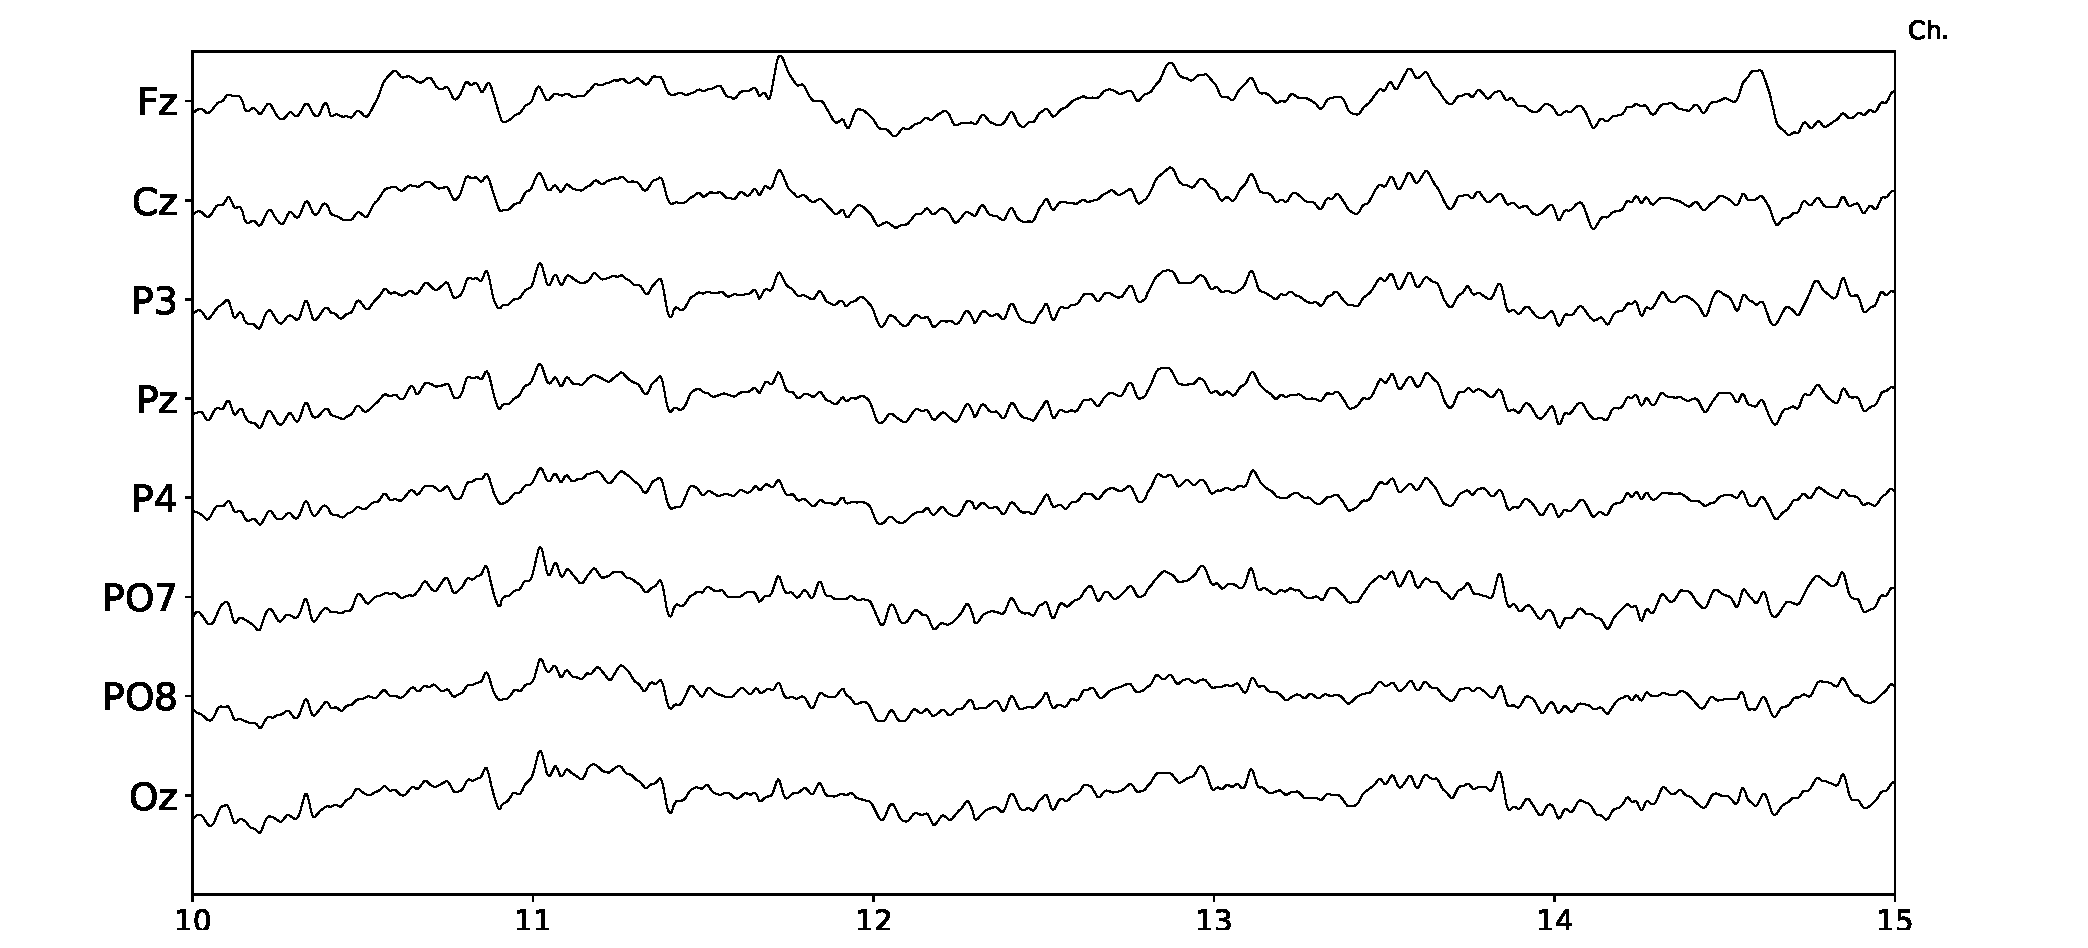
\includegraphics[height=6cm,width=12cm]{images/sampleeeg.eps}
\caption{Sample EEG signal obtained from g.Tec g.Nautilus.  Time axis is in seconds and five seconds are displayed.  The eight channels provided by this device are shown.}
\label{fig:sampleeeg}
\end{figure}

%locations.eps

The device that captures these small variations in potential differences over the scalp is called the Electroencephalograph.  Electrodes are located in predetermined positions over the head, usually embedded in saline solutions to facilitate the electrophysiological interface and are connected to a differential amplifier with a high gain which allows the measurement of tiny signals. Although initially analog devices were developed and used, nowadays digital versions connected directly to a computer are pervasive.  A detailed explanation on the particularities and modeling of EEG can be obtained from \citep{Jackson2014}, and a description of its electrophysiological aspects from \citep{Haberman2012}.

Overall, EEG signals can be described by their phase, amplitude,  frequency and \textit{waveform}.  The following elements regularly  characterize EEG signals:

\begin{itemize}
\item Artifacts:  These are signal sources which are not generated from the CNS, but can be detected from the EEG signal.  They are called endogeneous or physiological when they are generated from a biological source like face muscles, ocular movements, etc., and exogeneous or non-physiological when they have an external electromagnetic source like line induced currents or electromagnetic noise\citep{Weeda2012}.
\item Non-Stationarity: the statistical parameters that describe the EEG as a random process are not conserved through time, i.e. its mean and variance, and any other higher-order moments are not time-invariant \citep{Jansen1991}.
\item DC drift and trending: in EEG jargon, which is derived from concepts of electrical amplifiers theory, Direct Current (DC) refers to very low frequency components of the EEG signal which varies around a common center, usually the zero value.  DC drift means that this center value drifts in time.  Although sometimes considered as a nuisance that needs to get rid of, it is known that very important cognitive phenomena like Slow Cortical Potentials or Slow Activity Transients in infants do affect the drift and can be used to understand some particular brain functioning \cite{Schomer2010}.
\item Basal EEG activity: the EEG is the compound summation of myriads of electrical sources from the CNS.  These sources generate a baseline EEG which shows continuous activity with a small or null relation with any concurrent cognitive activity or task.
\item Inter-subject and intra-subject variability: EEG can be affected by the person's behavior like sleep hygiene, caffeine intake, smoking habit or alcohol intake previously to the signal measuring procedure \citep{Farzan2017}.
\end{itemize}

Regarding how the EEG activity can be related to an external stimulus that is affecting the subject, it can be considered as

\begin{itemize}
\item Spontaneous: generally treated as noise or basal EEG.
\item Evoked: activity that can be detected synchronously after some specific amount of time after the onset of the stimulus.  This is usually referred as time-locked.  In contrast to the previous one, it is often called Induced activity.
\end{itemize}

\noindent Additionally, according to the existence of a repeated rhythm, the EEG activity can be understood as

\begin{itemize}
\item Rhythmic: EEG activity consisting in waves of approximately constant frequency.  It is often abbreviated RA (regular rythmic activity). They are loosely classified by their frequencies, and their naming convention was derived from the original naming used by Hans Berger himself, and after Alpha Waves (10 Hz), it came Delta (4 Hz), Theta (4-7 Hz), Sigma (12-16 Hz), Beta (12-30 Hz) and Gamma (30-100 Hz).  
\item Arrhythmic: EEG activity in which no stable rhythms are present.  
\item Dysrhythmic: Rhythms and/or patterns of EEG activity that characteristically appear in patient groups and rarely seen in healthy subjects.
\end{itemize}

The number of electrodes and their positions over the scalp determines a \textbf{Spatial Structure}: signal elements can be generalized, focal or lateralized, depending on in which channel (i.e. electrode) they are found.

%Finally, indexes can be derived as  CFC, Cross Frequency Coupling,  Phase-Amplitude Coupling, Phase-Phase Coupling.


\subsection{EEG Waveform Characterization}

The shape of the signal, the waveform, can be defined as the graphed line that represents the signal's amplitude plotted against time. It can also be called EEG biomarker,  EEG pattern, signal shape, signal form and a morphological signal \citep{Jansen1991}.

The signal context is crucial for waveform characterization, both in a spatial and in a temporal domain \citep{Jansen1991}.  Depending on the context, some specific waveform can be considered as noise while in other cases is precisely the element which has a cognitive functional implication.

%aforegoing
%hitherto

%phenomenological, the signal is treated as a black box.

%Signal Morphology is not precisely defined in the literature but may refer to
%
%\begin{itemize}
%\item RA (regular rythmic activity) 
%\item low-voltage rapid activity 
%\item sharp waves
%\item longitudinal-bipolar and transverse- bipolar montages (Clinical EEG)
%\end{itemize}

A waveform can have a characteristic shape, a rising or falling phase, a pronounced plateau or it may be composed of ripples and wiggles. In order to describe them, they are characterized by its amplitude, the arch, whether they have (non)sinusoidal shape, by the presence of an oscillation or imitating a sawtooth (e.g. Motor Cortical Beta Oscillations).  The characterization by their sharpness is also common, particularly in Epilepsy, and they can also be identified by their resemblance to spikes (e.g. Spike-wave discharge).

Depictions may include subjective definitions of sharper, arch comb or wicket shape, rectangular, containing a decay phase or voltage rise, peaks and troughs, short term voltage change around each extrema in the raw trace.  Derived ratios and indexes can be used as well like peak and trough sharpness ratio, symmetry between rise and decay phase and slope ratio (steepness of the rise period to that of the adjacent decay period).  For instance,  wording like "Central trough is sharper and more negative that the adjacent troughs"~\citep{Cole2017} are common in the literature.

Other regular characterizations which are based on the waveform shape may encompass:

\begin{itemize}
\item Attenuation: Also called suppression or depression. Reduction of amplitude of EEG activity resulting from decreased voltage. When activity is attenuated by stimulation, it is said to have been "blocked" or to show "blocking".
\item Hypersynchrony: Seen as an increase in voltage and regularity of rhythmic activity, or within the alpha, beta, or theta range. The term suggest an increase in the number of neural elements contributing to the rhythm, or in the synchronization of different neurons with the same discharge pattern~\citep{Buzsaki2012}.
\item Paroxysmal: Activity that emerges from background with a rapid onset, reaching (usually) quite high voltage and ending with an abrupt return to lower voltage activity. 
\item Monomorphic: Activity appearing to be composed of one dominant waveform pattern.
\item Polymorphic: Activity composed of multiple frequencies that combine to form a complex waveform.
\item Transient: An isolated wave or pattern that is distinctly different from background activity. 
\end{itemize}

%  Define component, source and sensor space.

%\subsection{EEG Patterns}
%
%%The clinical EEG patterns are identified by the shape of waveform amplitude plotted against time.
%
%Non-exhaustive list of transient events
%Waveform characterization is of quite importance in terms of Event Related Potentials.  
%Determination of transient events, and particularly amplitude of different subcomponents, latency or even phase, has proved very importan concequences in terms of the different cognitive approach.
%
%%inverse problem is mathematically intractable Voytek 2009
%
%Oscillatory activity can also have their differente or distinctive waveforms.  Slow oscillations, which are assosiated with REM, sawtooth-shaped.
%Sleep spindles can also be considered oscilations and they have a distintinc form assosiated with stage 2 dream.
%Visual Cortical alpha and rolandic central mu waves arch-like structure (similar to the greek letter mu).  Slope Ratio.  Trough voltage remains contstant while peak voltage fluctuates.   Steep slopes,   Amplitude asymmetry 
%ponto-geniculo-occipital
%(PGO) waves.
%Rhythms in neural activity are observed across various temporal and spatial scales and are often
%referred to as oscillations (see Glossary) [1]. Traditionally, neural oscillations have been
%clustered into canonical frequency bands, including delta (1–4 Hz), theta (4–8 Hz), alpha (8–
%12 Hz), beta (15–30 Hz), gamma (30–90 Hz), and high gamma (>50 Hz). These bands roughly
%correspond to frequency ranges commonly observed in human electroencephalography (EEG)
%studies. Although they have been observed for nearly a century, recent theories suggest that
%these oscillations play an active role in neural communication.  Hippocampal theta oscillations, for example, are among the best-studied rhythms in the local field potential (LFP); they have a stereotyped sawtooth shape. In sleep research sleep 2 stage the background of KComplex and sleep spindles is theta waves
%
%%by application to Brain Computer Interfaces or EEG diagnosis (BCI a review, BCI Vidal 1973)
%
%
%
%%(e.g. FIRDA - Frontal Intermittent Rhythmic Delta) and posteriorly in children e.g. OIRDA - Occipital Intermittent Rhythmic Delta).
%
%%alpha dissapears when alerting by any mechanism (thinking, calculating)
%
%a) Spike: a transient with a pointed peak and a duration from 20 to under 70 msec.
%b) Sharp wave: a transient with a pointed peak and duration of 70-200 msec.
%
%Some initial works on EEG explored the idea to extend human capacities analyzing EEG waveforms  (automatic detection of k complexes), (A Waveform Analyzer Applied to the Human EEG) where a feature from amplitude and frequency of its signal and its derivative in time-domain is used.  Althought CASENET REFERENCe explored "waveform" structure they were purely based on spike detection based on feeding artificial neural networks.  
%
%ACA VA EL RESTO DE LOS METODOS (fujimori, PAA, etc).  Uchida 1999

The traditional clinical approach consists in analyzing the paper strip that is generated by the plot of the signal obtained from the device.  Expert technician and physicians analyze visually the plots looking for specific patterns that may give a hint of the underlying cognitive process or pathology.   Atlases and guidelines were created in order to help in the recognition of these complex patterns.   Even Video-electroencephalography scalp recordings are routinely used as a diagnostic tools \citep{Giagante2003} .  The clinical EEG research has also focused on temporal waveforms, and a whole branch of electrophenomenology has arisen around EEG \textit{graphoelements} \citep{Schomer2010}.  

Sleep Research has been studied in this way by performing Polysomnographic recordings (PSG)~\citep{Boostani2017,Rodenbeck2006}, where the different sleep stages are evaluated by visually marking waveforms or graphoelements in long-running electroencephalographic recordings, looking for patterns based on standardized guidelines~\citep{Dimitriadis2018}. Visual characterization includes the identification or classification of certain waveform components, or transient events, based on a subjective characterization (e.g. positive or negative peak polarity) or the location within the strip.  It is regular to establish an amplitude difference between different waveforms from which a relation between them is reckoned and a structured index is created (e.g. sleep K-Complex is well characterized based on rates between positive vs negative amplitude) \citep{Uchida1999}.  Other relevant EEG patterns for sleep stage scoring are alpha, theta, and delta waves,  sleep spindles, polysplindles, vertex sharp waves (VSW), and sawtooth waves (REM Sleep).

Moreover, EEG data acquisition is a key procedure during the assessment of patients with focal Epilepsy for potential seizure surgery, where the source of the seizure activity must be reliably identified. The onset of the Epileptic Seizure is defined as the first electrical change seen in the EEG rhythm which can be visually identified from the context and it is verified against any clinical sign indicating seizure onset.  The Interictal Epileptiform Discharges (IEDs) are visually identified from the paper strip, and they are also named according to their shape: spike, spike and wave or sharp-wave discharges\citep{EEGIntro}.  

Waveform characterization is the method in which analysis has been performed for Event Related Potentials.  Evoked Potentials (EPs) and Event Related Potentials (ERPs) are transient signal elements that may arise as a brain response to an external visual, tactile or auditory stimulus.  ERPs are regularly used to assess auditory response in infants.  They are extensively used and studied in Cognitive Neuroscience~\citep{Luck2005}.  ERPs are identified by their components which are recognizable signal shapes assigned to the observed waveform, that can be linked to some cognitive or measurable psychological process.   The P300 is one of the most studied ERP component in BCI because it can be used to implement a Speller application.  Hence, P300 ERPs are a target phenomena to study by automatic waveform recognition methods.

Table~\ref{tab:methods} shows a list of depictions used to describe waveforms in the surveyed literature.  Epilepsy has been described by the nature of oscillatory characterization of their waves, like ripples and wiggles, imitating sawtooths or by their geometric shape.  For ERPs on the other hand, more elaborate indexes has been provided establishing relations between signal components amplitudes.  Finally, in sleep studies and ICU research areas is where the most complex indexes has been derived, particularly coupling signal properties like phase, amplitude and frequency.

%The clinical EEG patterns are identified by the shape of waveform amplitude plotted against time.


%
%Non-exhaustive list of transient events
%

%Seizures captured in their entirety typically show progression from low-voltage, high-frequency spikes to high-voltage, low-fre- quency spike-and-slow wave activity, before stopping abruptly and being replaced by background slowing or suppression (Fig. 29.9). Usual morphologic features include typical rhythmic, gen- eralized, symmetric spike-and-waves or polyspikes and waves at 2 to 3.5 Hz; atypical spike and wave with lower frequency and less symmetry; multiple spike-and-wave (repetitive complexes of two or more spikes followed by a slow wave); and high-voltage, repetitive, rhythmic, focal or generalized delta activity with inter- mixed spikes, sharp waves, or sharp components (Fig. 29.24) (45). Diagnosis is more difficult when the seizure (or SE) pre- cedes the beginning of the tracing and continues beyond its end. In such cases, rhythmic sharp features, typically faster than 1 Hz, may be seen, often with variability.

%Finally, there are specific EEG patterns that can be used to determine Depth of anestisia. 

%The waveform of the EEG depends on the settings of the capturing device.  The most important part to consider is that of montage.  It could be bipolar or referencial.  The traditional convention, somehow maintained in neuro research, downward polarity was considered negative and upward deflection for negative (Knott, 1985)  It is of utmost importance to remark that  EEG waveforms represent the differential voltage between a given electrode and the recording reference. It is therefore clear that the choice of reference completely determines EEG waveforms (Lehmann, 1987; Dien, 1998), an important methodological consideration that all too often is still not recognized in the EEG literature. For example, recording with a vertex (Cz) reference would lead to small EEG deflections in the proximity of Cz due to potential synchronization of firing activities within closely spaced brain regions and volume propagation of the EEG signal. Similarly, recording with mastoid or linked ears montage would lead to rather small waveforms at electrodes positioned over temporal brain regions (Pivik et al., 1993). Digital EEG can be rereferenced offline.  

%
%BCI --> distinguishing the pertinent signal characteristics from extraneous content and representing them in a compact or menaingful form, amenable to interpretation by a human or computer (Wolpaw and Wolpaw)

%Transient phenomena allows also to record occurrence and temporal sequence (mimicking spike analysis in neuro reserach)

%The traditional approach do not consider waveform even though the brain oscilations are in general nonsinusoidal (reference)
% Waveform characterization, on the other hand, has been extensively used in artifact detection and averaging.

% Non-exhaustive list of EEG Waveforms, their phenomena and the literature reference where they are described.

\begin{table}[H]
\caption{EEG waveforms descriptions found in the surveyed literature.}
\centering
%% \tablesize{} %% You can specify the fontsize here, e.g.  \tablesize{\footnotesize}. If commented out \small will be used.
\begin{tabular}{ccc}
\toprule
\textbf{Method}	& \textbf{Phenomena} & \textbf{Reference}	\\
\midrule
Positive Rounded Component                    & $\alpha$-Waves, Epilepsy & \citep{Schomer2010,Tatum2008} \\
Rising and Falling Phase      & Epilepsy &  \citep{Thakor2004,Tatum2008} \\
Terminal plateau      & Epilepsy &  \citep{Thakor2004} \\
Ripples and Wiggles     & Epilepsy, ERP &  \citep{EEGIntro, Thakor2004,Cacioppo2007,Kappenman2012} \\
Sinusoidal Shape        & Epilepsy &  \citep{Cacioppo2007,Tatum2008,Ouyang2017,Kappenman2012,Cole2017} \\
Sawtooth                     & Motor Imagery, Sleep &  \citep{EEGIntro,Rodenbeck2006,Tatum2008} \\
Sharpness or Spike-like     & Epilepsy &  \citep{Thakor2004,Hartman2005,Sanei2007,EEGIntro} \\
Rectangular     & Epilepsy &  \citep{Thakor2004,Cole2017} \\
Line length       & Anomaly Detection & \citep{Wulsin2011} \\
Root Mean Square & Anomaly Detection & \citep{Wulsin2011} \\
Wicket Shape     & Epilepsy &  \citep{EEGIntro,Hartman2005,Sanei2007,Tatum2008,Schomer2010,Cole2017} \\
Peak and Trough Sharpness Ratio     & Epilepsy &  \citep{Hartman2005,Sanei2007,Lawrence2010,Cole2017} \\
Symmetry between rise and decay phase     & Epilepsy &  \citep{Hartman2005,Cole2017} \\
Slope Ratio    & Sleep &  \citep{Subha2010} \\
Positive/Negative Peak Amplitude & ERP & \citep{Thakor2004,Hartman2005,Tatum2008,Mak2012,MullerPutz2015,Cole2017} \\
Positive vs Negative Ratio    & Sleep K-Complex &  \citep{EEGIntro} \\
Base-to-Peak Amplitude     & ERP  &  \citep{Cole2017} \\
Peak-to-Peak Amplitude     & ERP  &  \citep{Wulsin2011,Mak2012} \\
Positive/Negative Peak Latency                                 & ERP  & \citep{Mak2012}  \\
Integrated Activity               & ERP, Epilepsy,ICU & \citep{Wulsin2011,Uchida1999, Shah2015} \\
Cross-Correlation                & ERP, Epilepsy, Sleep & \citep{Cacioppo2007, Shah2015} \\
Coupling \\ Cross Frequency,  Phase-Amplitude, Phase-Phase     & Sleep & \citep{Cole2017} \\
Period Amplitude Analysis  & ERP, Epilepsy & \citep{Uchida1999,Cacioppo2007, Shah2015} \\
\bottomrule
\end{tabular}
\label{tab:methods}
\end{table}


\section{Materials and Methods}

The search of methods based on waveforms is conducted by following the PRISMA~\citep{Moher2009} guidelines.  Search is performed on Google Scholar, Semantic Web and IEEE Xplore search engines by the terms "Waveforms" OR "Shape" OR "Morphology" OR "Visual inspection" + "EEG".

The following criteria is proposed to identify methods which are based on the signal's waveform:

\begin{enumerate}
\item The analysis considers the shape of the plot of the signal.
\item The pattern can be identified and verified by visual inspection.
\item The pattern matching is performed in time-domain.
\item The method encompass a feature extraction procedure.
\item The feature extraction procedure allows to create a template dictionary.
\end{enumerate}

As described in \citep{allen2004signal} the Pattern Matching problem in Signal processing is finding a signal given the region that best describes the structure of the prototype signal template.   On the other hand, a \textit{feature} is a meaningful quantification, usually a multidimensional vector, that synthesize the information of a given signal or signal segment~\citep{WolpawJonathanR2012}.   

\subsection{EEG Waveform Analysis Algorithms}
\label{Algorithms}

Shape or waveform analysis methods are considered as nonparametric methods.  They explore signal's time-domain metrics or even derive more complex indexes or features from it \citep{Thakor2009}. 

One of the earliest approach to automatically process EEG data is the Peak Picking method.  Although of limited usability, peak picking has been used to determine latency of transient events in EEG \citep{Jaskowski2000,Zhang2011}.  Straightforward in its implementation, it consists in assigning a component to a simple waveform element based on the expected location of its more prominent deflection \citep{Ouyang2017}.  
Of regular use in ERP Research, the name of many of the EEG features reference directly a peak within the component, e.g. P300 or P3a P3b or N100.  This leads to a natural way to classify them visually by selecting appropriate peaks and matching their positions and amplitudes in an orderly manner.  The letter provides the polarity (Positive or Negative) and the numbering shows the time referencing the stimulus onset, or the ordinal position of each peak (first, second, etc). 

%Evoked Potentials (EPs) and Event Related Potentials (ERPs) are transient component that may arise as a brain response to an external visual, tactile or auditory stimulus.  Particularly, ERPs are regularly used to assess auditory response in infants. They are characterized in this manner, where the name of many of the EEG features evoke directly a peak within the waveform, e.g. P300 or P3a P3b or N100.  This leads to a natural procedure to classify them visually by selecting appropriate peaks and matching their positions and amplitudes in an orderly manner.  The letter provides the polarity (Positive or Negative) and the numbering shows the time referencing the stimulus onset, or the ordinal position of each peak (first, second, etc).   

A related method is used in \citep{Alvarado-Gonzalez2016} where the area under the curve of the EEG is sumarized to derive a feature.  This was even used in the seminal work of Farwell and Donchin on P300 \citep{Farwell1988,WolpawJonathanR2012}. Additionally, a logarithmic graph of the peak-to-peak amplitude which is called amplitude integrated EEG (aEEG) \citep{Shah2015} is used nowadays in Neonatal Intensive Care Units.

Other works on EEG explored the idea to extend human capacities analyzing EEG waveforms \citep{Klein1976} where a feature derived from the amplitude and frequency of its signal and its derivative in time-domain is used.  Moreover, other approaches explored the use of Mathematical Morphology \citep{Yamaguchi2009}, where the time-domain structure of contractions and dilations were studied. Finally the proposals of Burch, Fujimori, Uchida and the Period Amplitude Analysis (PAA) \citep{Uchida1996} algorithm are few of the earliest depictions where the idea of capturing the shape of the signal were established.

%Althought CASENET REFERENCe explored "waveform" structure they were purely based on spike detection based on feeding artificial neural networks.  

 %(fujimori, PAA, etc).  Uchida 1999

%\subsubsection{Averaging Methods}
%
%The methods that allow to identified waveforms are used to determine different alignments while averaging epochs.
%
%This long-standing problem has been tackled from different perspectives.  Woody's Template Matching is perhaps the best effort as well as Pham, and Tuan and others EML.
%
%Dictionary, template based method.  Many do not consider the waveform, albeit they do use a set of templates obtained from a dictionary.
%
%Cross Covariance with Template or Cross Correlation or ACF: Autocorrelation Function: PHAM METHOD
%
%Applying a FIR filter with templates 
%
%Krusienski et al 2007
%Serby et al 2005
%
%extended to wavelent analysis.
%
%Dynamic Time Warping and other Warp Averaging methods were also used.
%
%Wrapping Analysis
%
%Warp averaging

According to the defined criteria, the algorithms that will be evaluated are as follows:

\begin{itemize}
\item Matching Pursuit
\item Permutation Entropy
\item Slope Horizontal Chain Code
\item Scale Invariant Feature Transform
%\item Merging of Increasing and Decreasing Sequences
%\item Local Binary Patterns (1-D LNBP, 1D-LBP and LBP)
\end{itemize}

All these methods provide a feature $ f $~\footnote{The notation $f=\{f_i\}_{1}^{n} $ or $f=\{f_i\}_{i \in J}^{} $  will be used to describe the concatenation of scalar values to form a multidimensional feature vector $f=\{f_1,f_2,...,f_n\}$.}  that can be used as a template. These algorithms are based on metrics that are extracted from the shape of the single channel digital EEG signal $x(n)$, with $n$ varying from $1$ to the length $N$ of the EEG segment in sample points.  These features are used to create dictionaries or template databases.  Finally, these templates provide the basis for the pattern matching algorithm and offline classification. These algorithm were implemented on MATLAB 2014a (Mathworks Inc., Natick, MA, USA).  To maintain reproducibility, the data and the source code has been made available in the online repository of the Code Ocean platform under the name \textit{EEGWave}.

\subsection{Matching Pursuit - MP 1 and MP 2}

\textit{Pursuit} algorithms refer, in their many variants, as blind source separation \citep{Vincent2010} techniques that assume the EEG signal as a linear combination of different sparse sources extracted from a template's dictionaries.  Matching Pursuit \textit{MP}~\citep{Mallat1993}, the most representative of these algorithms, is a greedy variant that decomposes a signal into a linear combination of waveforms, called atoms, that are well localized in time and frequency \citep{ChandranKS2016}.  Given a signal, this optimization technique, tries to find the indexes of $m$ atoms and their weights (contributions) that minimize,


\begin{equation}
\varepsilon =  \left\lVert   x(n) - \sum_{i=1}^{m} w_i g_{i}(n)   \right\rVert
\label{eq:mperror}
\end{equation}

\noindent which is the error between the signal and its approximation constructed by the weighted $w_i$ atoms $g_{i}$, and calculating the euclidean norm ${\left\lVert \cdot \right\rVert}_{2}$.  The algorithm goes by first setting the approximating signal $\tilde{x}_{0}$  as the original signal itself,  

\begin{equation}
\tilde{x}_{0}(n) = x(n)
\label{eq:mp2}
\end{equation}

\noindent and setting the iterative counter $k$ as $1$. Hence, it searches recurrently the best template out of the dictionary  that matches current approximation.  

\begin{equation}
g_{k} = \arg \max_{g_{i}} \left\lvert  \sum_{n=1}^{N} \tilde{x}_{k-1}(n) \; g_{i}(n) \right\rvert 
\label{eq:mp3}
\end{equation}

\noindent where $g_{i}$ are all the available scaled, translated and modulated atoms from the dictionary.  The operation $\left\lvert \cdot \right\rvert$ corresponds to the absolute value of the inner product.  This step determines the atom selection process, and their contribution is calculated based on 

%The operation $\left\lvert < \cdot,\cdot > \right\rvert$ corresponds to the absolute value of the inner product. 


\begin{equation}
w_{k} =  \frac{\sum_{n=1}^{N} \tilde{x}_{k-1}(n) \; g_{k}(n)}{  {\left\lVert  g_{k} \right\rVert}^{2} }
\label{eq:mp4}
\end{equation}

\noindent with $k$ representing the index of the selected atom $g_{k}$ and $\left\lVert \cdot \right\rVert$ its euclidean norm.  Finally the contribution of each atom is subtracted from the next approximation~\citep{Cohen2014,Sanei2007, Mallat1993}

\begin{equation}
\tilde{x}_{k}(n)=  \tilde{x}_{k-1}(n) - w_{k} g_{k} (n)
\label{eq:mp5}
\end{equation}

The stopping criteria can be established based on a limiting threshold on Equation \ref{eq:mperror} or based on a predetermined number of steps and selected atoms.  Two variants of this algorithm are evaluated. In \textit{MP 1} the dictionary is constructed with the normalized templates directly extracted from the real signal segments which is a straightforward implementation of the pattern matching technique.  In \textit{MP 2} the coefficients of Daubechies least-asymetric wavelet with 2 vanishing moments atoms are used to construct the dictionary~\citep{Vareka2012}.  For the first version, the matching against the template is evaluated according to Equation \ref{eq:mperror} directly, whereas for the latter each feature is crafted by decomposing the signal in its coefficients and building, an eventually sparse, vector with them:

\begin{equation}
f =  {\bigg \{ w_{i} \bigg \}}_{1}^{D} 
\label{eq:mp6}
\end{equation}

\noindent where $D$ is the size of the dictionary.  

%On the other hand, Morphological Component Analysis is a variant form of Blind Source Separation which can be considered the extension of Matching Pursuit algorithm. (cita a esa parte del paper).


\subsection{Permutation Entropy - PE}

Bond and Pompe Permutation Entropy has been extensively used in EEG processing, with applications on Anesthesia, Sleep Stage evaluation and increasingly for Epilepsy pre-ictal detection \citep{Bandt2002}.  This method generates a code based on the orderly arrangement of sequential samples, and then derives a metric which is based on the number of times each sequence is found along the signal.  This numeric value can be calculated as information entropy~\citep{Nicolaou2010}. Let's consider a signal on a window of length $W$ represented by the sample points

\begin{equation}
(x_1,x_2,...,x_{W})
\label{eq:pesignal}
\end{equation}

\noindent and resampled by $\tau$ intervals, starting from the sampling point $n$, doing

\begin{equation}
(x_n,x_{n+\tau},x_{n+2 \tau}...,x_{n+(m-1)\tau}).
\label{eq:pe2}
\end{equation}

This sequence is of order $m$, which is the number of sample points used to derive the ordinal element called $\pi$. There are $m!$ ways in which this sequence can be orderly arranged, according to the position that each sample point holds within the sequence in a strict order relationship.  For example if $m=3$, and the first sample point is the bigger, the second is the smaller and the third one is in the middle, the ordinal element $\pi$ corresponds to $(3,1,2)$. Thus, along the signal window there can be at most $k$ different ordinal (and overlapping) elements $\pi_{s}$

\begin{equation}
(\pi_{1},\pi_{2},...,\pi_{k})
\label{eq:pe3}
\end{equation}

\noindent with $k = W-(m-1) \tau$.  The probability density function \textit{pdf} for all the available permutations of order $m$ should be $ \textbf{p} = (p_1,p_2,...,p_{m!}) $ with $ \sum_{i=1}^{m!} p_{i} = 1 $.

Hence, the time series window is mapped to a new set of $k$ ordinal elements, and the \textit{pdf} can be calculated by the empirical permutation entropy,

\begin{equation}
p_i = \frac{1}{k} \sum_{s=1}^{k} \left[ \pi_{s} = \pi_{i} \right]
\label{eq:pe4}
\end{equation}

\noindent with $1 \leq i \leq m!$. The Iverson Bracket $ \left[ \cdot \right] $ resolves to $1$ when their logical proposition argument is true, $0$ otherwise. Therefore, for each $i$ only those ordinal elements $\pi_{s}$ that were effectively found along the signal are counted to estimate $p_i$, and zero elsewhere.  The empirical permutation entropy can be calculated from the histogram as,

\begin{equation}
H(\textbf{p}) = \sum_{i=1}^{m!} p_{i} \; log \frac{1}{p_{i}}.
\label{eq:pe5}
\end{equation}

The implemented code was derived from~\citep{Unakafova2013}, and the model description from \citep{Berger2017}.  This procedure produces a scalar number for the given signal window of size $W$.  To derive a feature, a sliding window procedure must be implemented to cover an entire segment of length $N$.  Thus, the length of the feature is $N - (W + \tau (m - 1))$.

\begin{equation}
f =  {\bigg \{ H(\textbf{p})_{u} \bigg \}}_{W + \tau  m}^{N}.
\label{eq:pe6}
\end{equation}

\noindent with $u$ varying on a sample by sample basis along the signal, starting from the specified index.

\subsection{Slope Horizontal Chain Code - SHCC}

This algorithm~\citep{Alvarado-Gonzalez2016} proceeds by generating a coding scheme from a sequence of sample points. This encoding is based on the angle between the horizontal line on a 2D-plane and any segment produced by two consecutive sample points, regarding them as coordinates on that plane.  

A signal of length $N$, can be represented by a list of ordered-pairs $e$,

\begin{equation}
e = \left[ (x,y)_{1}, (x,y)_{2}, ..., (x,y)_{N} \right]
\label{eq:shccdelta}
\end{equation}

\noindent and it can be divided into $G$ different blocks.  These blocks are obtained by resampling the original signal from the index 

\begin{equation}
G = \lfloor n + ( m \Delta ) + 0.5 \rfloor
\label{eq:shcc2}
\end{equation}

\noindent with $n$ being the original sampling index on $ 1 \leq n \leq N $ and $\lfloor \cdot \rfloor$ being the floor operation, i.e. rounding of the number argument to the closest smaller integer number.  On the other hand, $\Delta$ can be obtained by

\begin{equation}
\Delta = \bigg \lceil \frac{N}{G+1} \bigg \rceil
\label{eq:shcc3}
\end{equation}

\noindent with $ G < N $ and using instead $\lceil \cdot \rceil$ as the ceil operation, the rounding to the closest bigger integer number. Lastly, the value $m$ can be derived from

\begin{equation}
m = sign \bigg (  \frac{N-1}{\Delta} \bigg )  \bigg \lfloor \left\lvert \frac{N-1}{\Delta} \right\lvert \bigg \rfloor.
\label{eq:shcc4}
\end{equation}

This resampling produces a new sequence of values,

\begin{equation}
e' = \left[ (x',y')_{1}, ...,(x',y')_{s}, ..., (x',y')_{G} \right].
\label{eq:shcc5}
\end{equation}

The next step is the normalization of each ordered-pair as vectors $\textbf{x'} = (x'_{1},...,x'_{G})$ and $\textbf{y'} = (y'_{1},...,y'_{G})$ according to

\begin{equation}
\hat{\textbf{x}} = \frac{\textbf{x'} - \min(\textbf{x'}) \textbf{1} }{\max(\textbf{x'}) - \min(\textbf{x'})} 
\label{eq:shcc6}
\end{equation}

\begin{equation}
\hat{\textbf{y}} = \frac{ \textbf{y'} - \min(\textbf{y'}) \textbf{1}}{\max(\textbf{y'}) - \min(\textbf{y'})} 
\label{eq:shcc7}
\end{equation}

\noindent with $\textbf{1}$ being the vector of length $G$ with all their components equal to $1$.  Hence, the scalar components $\hat{x}_{s}$ of $\hat{\textbf{x}}$, and $\hat{y}_{s}$ of $\hat{\textbf{y}}$, with $s$ varying between $1$ and $G$ are effectively normalized to $\hat{x}_{s},\hat{y}_{s} \in [0,1]$. \\

Finally, the feature is constructed by calculating the point-to-point slope against the horizontal plane,

\begin{equation}
f = \bigg \{  \frac{\hat{y}_{s}-\hat{y}_{s-1}}{\hat{x}_{s}-\hat{x}_{s-1}}  \bigg \}_{2}^{G} 
\label{eq:shcc8}
\end{equation}


\subsection{Scale Invariant Feature Transform - SIFT}

SIFT~\citep{Lowe2004} is a very successful feature extraction technique from Computer Vision .  It has a biomimetic inspiration on how the visual cortex analyze images based on orientations~\citep{Edelman1997}.  This method has been used in \citep{Ramele2016} to analyze EEG signals based on their plots on 2D images.

The first step of the algorithm is the plot generation based on single-channel EEG segments $ x(n) $.  Hence, this signal is normalized by the z-score~\citep{Zhang2013}: 

\begin{equation}
\tilde{x}(n) = \left\lfloor \frac{\delta ( x(n) - \bar{x})}{\sigma_{x}} \right\rceil 
\label{eq:sift1}
\end{equation}

\noindent with $\delta$ being the signal magnification factor and $\bar{x}$ and $\sigma_{x}$, the mean and standard deviation of $x$ on the signal segment.  The width of the image is determined based on the $1$-second length size of the segment in sample units. This corresponds to the sampling frequency $F_s$ of the EEG signal segment. The width is adjusted by multiplying by the magnification factor $\delta$, 

\begin{equation}
w = \delta \; F_s
\label{eq:sift2}
\end{equation}

\noindent whereas the height is calculated based on the peak-to-peak amplitude of the signal within the segment,

\begin{equation}
h = \max_{n} \tilde{x}(n) - \min_{n} \tilde{x}(n).
\label{eq:sift4}
\end{equation}

Equation \ref{eq:sift5} determines the vertical position of the image where the signal's zero value will be located.

\begin{equation}
z = \left\lfloor \frac{h}{2} \right\rfloor - \left\lfloor \frac{\max_{n} \tilde{x}(n) + \min_{n} \tilde{x}(n)}{2} \right\rfloor.
\label{eq:sift5}
\end{equation}

Finally, a binary, black-and-white image plot is generated based on

\begin{equation}
I(z_1,z_2) = \left\{ \begin{array}{rl}
255 & \text{if} \,  z_1 = \delta \  n; \! z_2 = \tilde{x}(n) + z \\
0   & \mbox{otherwise}
\end{array}\right.
\label{eq:sift6}
\end{equation}

\noindent where $z_1$ and $z_2$ are the image coordinates values, $255$ represents white and $0$ is the background black color of the plot.  These points are interpolated using the Bresenham algorithm~\citep{Ramele2016}.

Once the plot is generated, its center is used to localize the center of the SIFT patch. This region of the image, where the signal's most important salient waveform should be located, is divided in a grid of $4 x 4$ block and the bidimensional gradient vectors are calculated on each one of them.  Therefore, for each block within the patch, a histogram of the gradient orientations, 8 circular orientations, are calculated.  This histogram is concatenated for all the 16 blocks and a feature is thus formed:

\begin{equation}
f = {\bigg \{ \bigg \{  \bigg \{ h(i,j,\theta) \bigg \}_{i \in I }  \bigg \}_{j \in I} \bigg \}_{\theta \in \Theta} }
\label{eq:sift7}
\end{equation}

\noindent with $i$ and $j$ varying belonging to $I = \{ 0,1,2,3 \} $ localizing the 16 blocks within the grid. The angles $\theta$ that belong to $\Theta$ are the eight possible equidistant values between $0$ and $315$.  This vector is normalized, clamped to $0.2$, and re-normalized again.   Details of the method can be found on \citep{Ramele2016,Lowe2004}.  It was implemented using the VLFeat  \citep{Vedaldi2010} public Computer Vision libraries.

%\subsection{Merger of Increasing and Decreasing Sequences}

%Stepwise downsampling 

\subsection{Experimental Protocol}
\label{Experimental}

Farwell and Donchin P300 Speller \citep{Farwell1988,Rakotomamonjy2008} is one the most used BCI paradigms to implement a thought translation device and to send commands to a computer in the form of selected letters, similar to typing on a virtual keyboard.  This procedure exploits a cognitive phenomena raised by the oddball paradigm: along the EEG trace of a person which is focusing on a sequence of two different visual flashing stimulus, a particular and distinctive transient component is found each time the expected stimulus flashes.  This is cleverly utilized in the P300 Speller, where rows and columns of a 6x6 matrix flashes randomly but only the flashing of a column or row where the letter that a user is focusing will trigger concurrently the P300 ERP along the EEG trace.

In order to verify this in a controlled procedure, a real P300 ERP template, obtained from a public dataset, is superimposed into a distinct EEG stream.  This trace was experimentally obtained by a subject which was observing the flashing of the stimulus matrix during a P300 Speller procedure but did not engage in focusing on any letter in particular. Everything is there, except the P300 ERP component. Along the EEG stream, the markers information was used to localize the \textit{True} segments where the P300 should have been found, and those timing locations are used to superimpose the extracted ERP waveform.  By implementing this pseudo-real approach, it is possible to effectively control null-signals and to adjust the shape of this evoked potential in accordance to similar procedures used in other works \citep{Ouyang2017,Jaskowski2000,QuianQuiroga2003}.

The experiments are as follows:

\begin{itemize}
\item Experiment 1 - Letter Identification Performance: the letter identification performance of each one of these methods on the artificially generated pseudo-real dataset.
\item Experiment 2 - Latency Noise:  Instead of superimposing the P300 ERP over the EEG trace at the exact locations where stimulus onsets are situated, an artificial latency lag is added.  The lagging value is picked from a uniform distribution $U(0,0.4)$ [s] ranging from $0$ to $0.4$ of the $1s$ segment size~\citep{DaPelo2018}.
\item Experiment 3 - Component Amplitude Noise: the amplitude of the main P3b component of the ERP template is randomly altered.  This component is defined to be located from the stimulus onset between $148$ ms up to $996$ ms which is around $840$ ms long.  This waveform element, multiplied by a gain factor, is subtracted from the original template.  This gain factor between $0$ and $1$ is drawn from a uniform distribution $U(0,1)$.  Additionally this subtracted waveform is multiplied by a Gaussian window with a support of the same length~\citep{Harris1978}.  This avoids adding any discontinuity into the artificial generated signal.
\end{itemize}

The classification method Support Vector Machine SVM with a linear kernel, is added for comparison as control using a feature $f$ constructed by normalizing the signal on each channel~\citep{Krusienski2006}.  This method has been proved efficient in decoding P300 in several BCI Competitions~\citep{Kaper2004}. 

All these experiments are executed using cross validation procedure dividing the letter to spell in two sets, preserving the structure of the letter identification trials. Spelling letters are scrambled while the order and group of each intensification sequence is preserved.

Finally the performance at letter identifications for these same methods is evaluated by performing an offline BCI Simulation on the Dataset IIb of the BCI Competition II (2003)~\citep{Blankertz2002}.  The protocol of this dataset is very similar to what was used to obtain the pseudo-real dataset.  The sampling frequency of this dataset is $240$, the number of letters are $73$ where the first $42$ are used to create the template dictionary for all the methods and the remaining $31$ are used to test the character recognition rate performance.  Additionally, in this dataset the number of available intensification number sequences is $15$.  

\subsubsection{Pseudo-Real Dataset Generation}

\paragraph{Passive Modality}

In this case the template ERP is acquired from the Subject Number $8$ of the public dataset 008-2014~\citep{Riccio2013} published on the BNCI-Horizon website \citep{Brunner2014} by IRCCS Fondazione Santa Lucia. Segments from the EEG signal containing the ERP are extracted for the trial number $2$, and they are point-to-point coherently averaged.  This P300 ERP can be seen in Figure  \ref{fig:erptemplate1}.  This template is selected due to its shape which more closely resemble the prototypical P300 waveform~\citep{Rao2013,Clerc2016}.

An EEG stream with null-P300 signal is obtained by the following procedure: 
Four (4) participants are recruited voluntarily and the experiment is conducted anonymously in accordance with the Declaration of Helsinki published by the World Health Organization.  No monetary compensation is handed out and they agree and sign a written informed consent.  This study is approved by the \textit{Departamento de Investigación y Doctorado, Instituto Tecnológico de Buenos Aires (ITBA)}.  The participants are healthy and have normal or corrected-to-normal vision and no history of neurological disorders. These voluntary subjects are aged between 20-40 years old.  EEG data is collected in a single recording session. Each subject is seated in a comfortable chair, with her/his vision aligned to a computer screen located one meter in front of her/him.  The handling and processing of the data and stimuli is conducted by the OpenVibe platform~\citep{Renard2010}.  Gel-based active electrodes (g.LADYbird, g.Tec, Austria) are used on locations Fz, Cz, Pz, Oz, P3,P4, PO7 and PO8 according to the 10-20 international system.  Reference is set to the right ear lobe and ground is preset as the AFz position.   Sampling frequency is set to 250 Hz.

All participants are instructed to passively watch the flashing screen while not focusing on any particular letter.  None of them have any experience with a BCI device.  A questionnaire is handed out at the end of the experiment with questions about how the participant felt during it, without giving more details.  

%This P300 Speller protocol consist in the flashing of 35 trails of 35 letters (7 words of 5 letter) where the intensification sequence of 6 rows and 6 columns is repeated 10 times for each letter.  More details can be found on the published work of \citep{Riccio2013}.

Figure~\ref{fig:gains} shows a $5s$ sample of the EEG trace obtained with the MNE library~\citep{Gramfort2013}.  Channel $S$ represents the twelve different stimulus markers (columns or rows) while channel $L$ represent the label (\textit{True} vs \textit{False}).  Labels are represented by square signals.  \textit{False} segments are marked with single amplitude square signals while \textit{True} segments are identified by double-amplitude square signals.  Subfigure (a) shows the signals before the ERP template is superimposed while subfigure (b) shows the same signals with the superimposed ERP template.  At first-sight, differences are really hard to spot visually.  Subfigures (c) and (d) show only one second of channels Cz and L from the same segment.  The superimposed ERP can be devised enclosed by the vertical bars, around $31.5$s, where in (d) the peak is slightly bigger.  Figure~\ref{fig:gaincheck} shows the obtained ensemble average ERPs as result of superimposing the template signal into the EEG stream, time-locked to the stimulus onset.   These 12 point-to-point averaged segments correspond to the first trial of the EEG stream.

%The original signal-to-noise ratio was calculated as Hue 2010.

\begin{figure}[H]
\centering
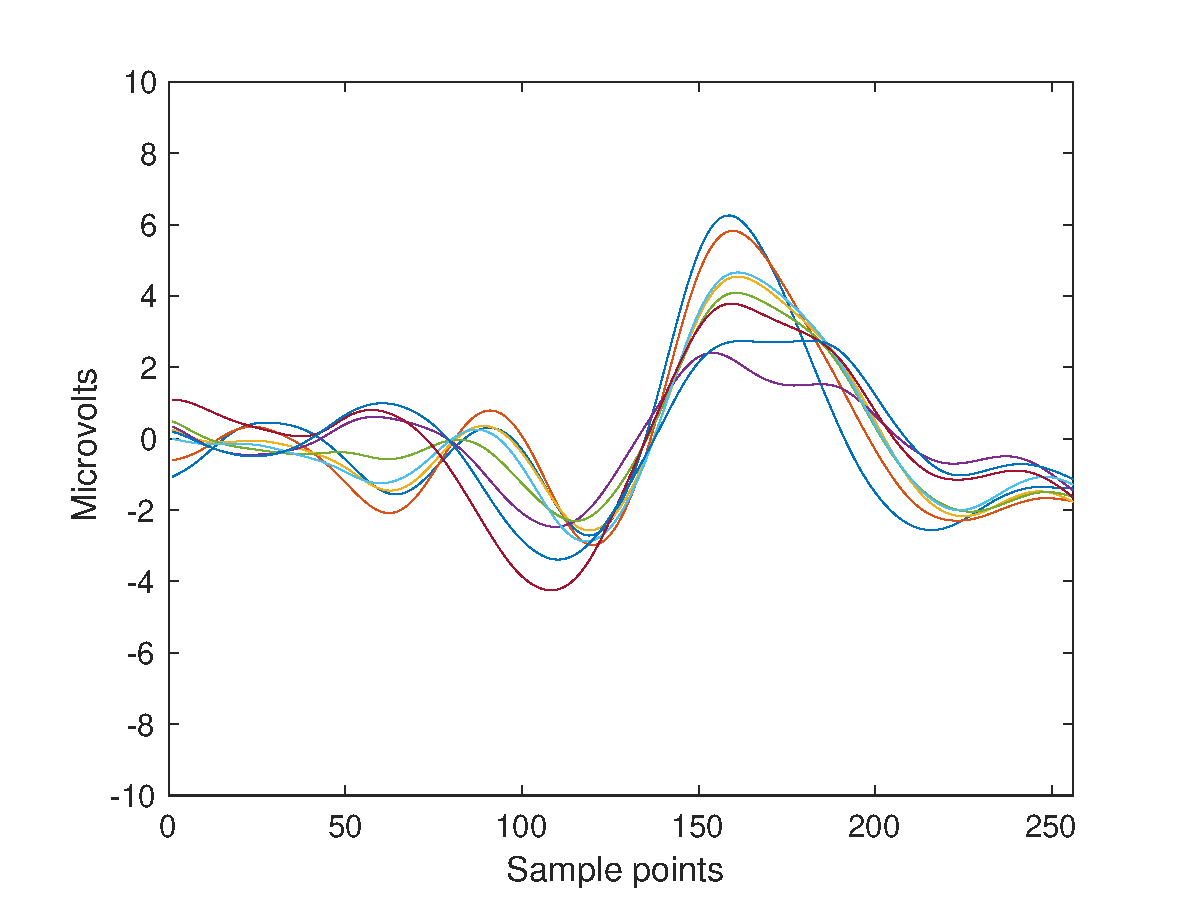
\includegraphics[width=12cm]{images/erptemplate1.eps}
\caption{ERP Template obtained from the coherent point-to-point ensemble average from the signals of Subject Number Eight of the BNCI Horizon public dataset 008-2014. The template is $1s$ long which is 256 sample points, and the eight channels are superimposed with different colors.  The P3b component can be seen around the sample index $150$ and $200$.}
\label{fig:erptemplate1}
\end{figure}

\begin{figure}[htb]
\centering
\subfigure[EEG trace of the original signal.]{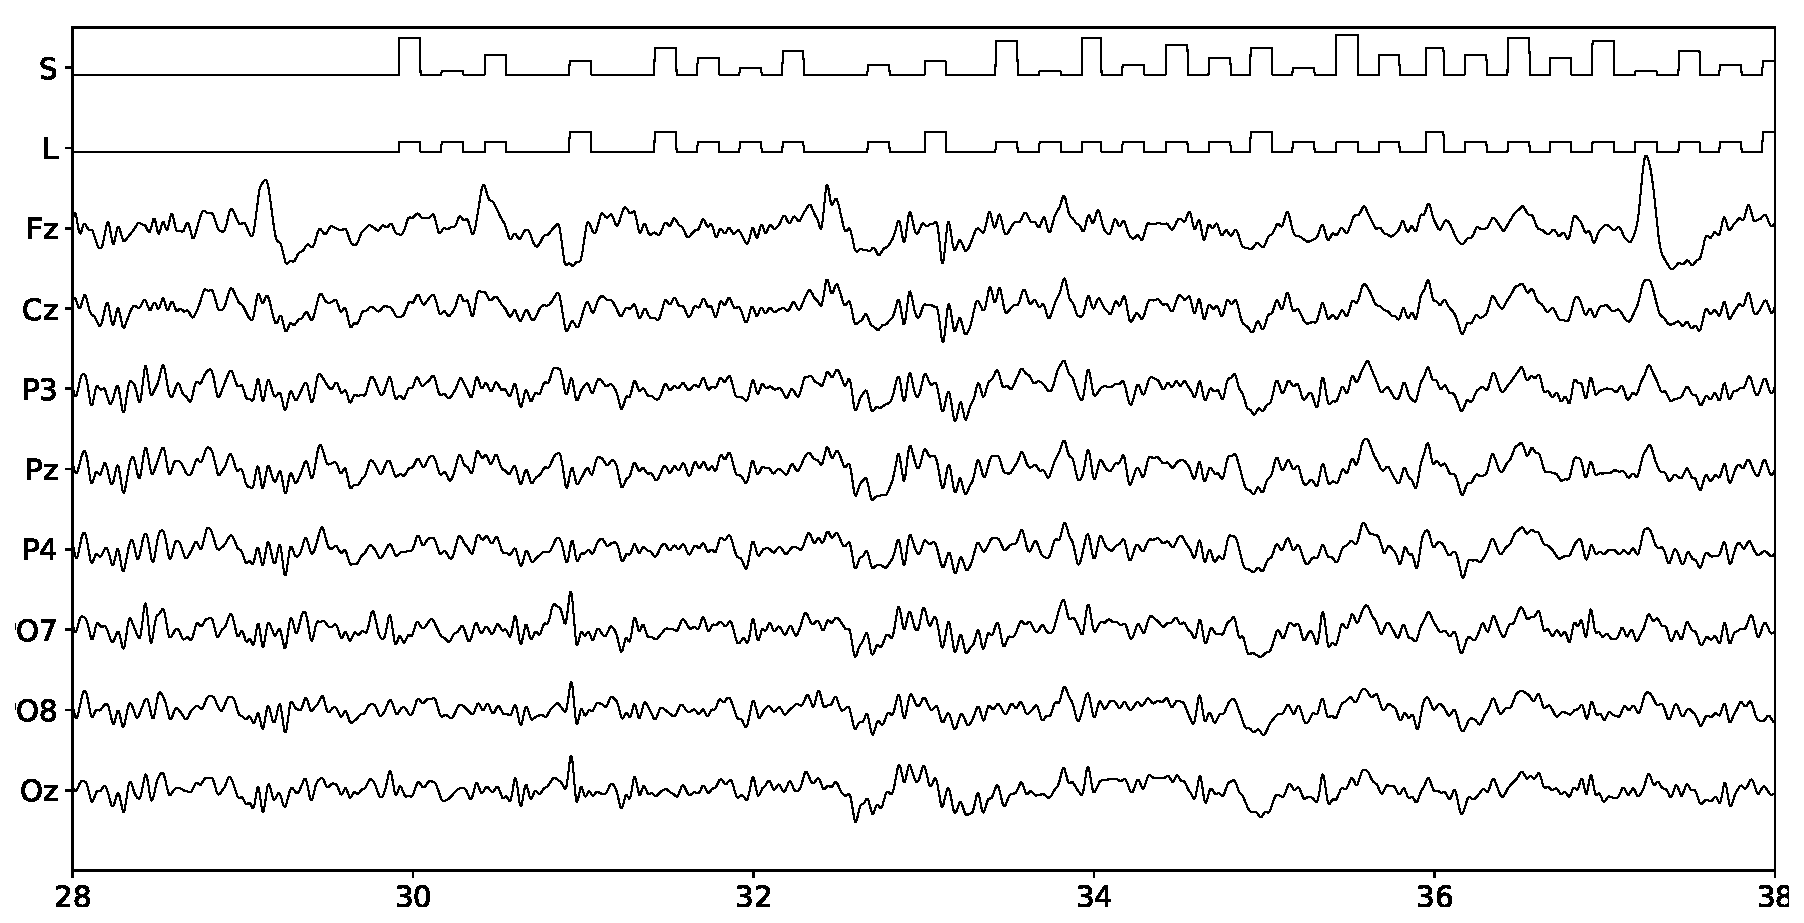
\includegraphics[width=.45\linewidth]{images/nogain.eps}}
\subfigure[The same eight-channel signal segment with the superimposed template.]{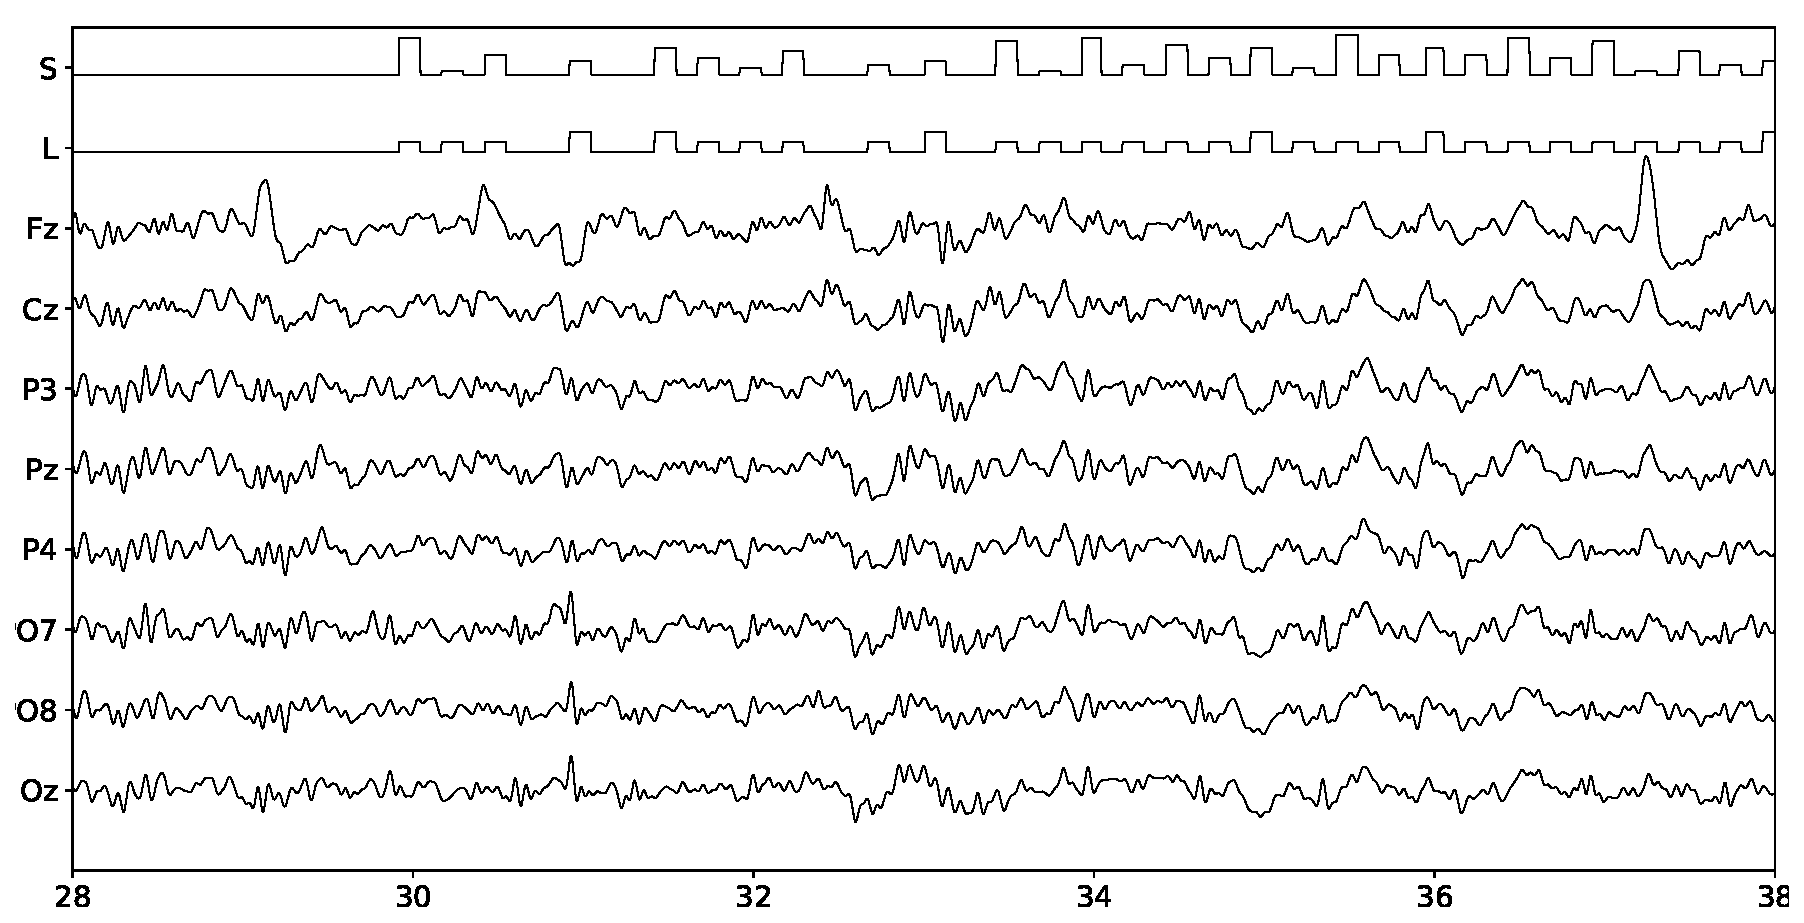
\includegraphics[width=.45\linewidth]{images/singlegain.eps}}
\subfigure[EEG sample of Cz and L channel of the original EEG trace.]{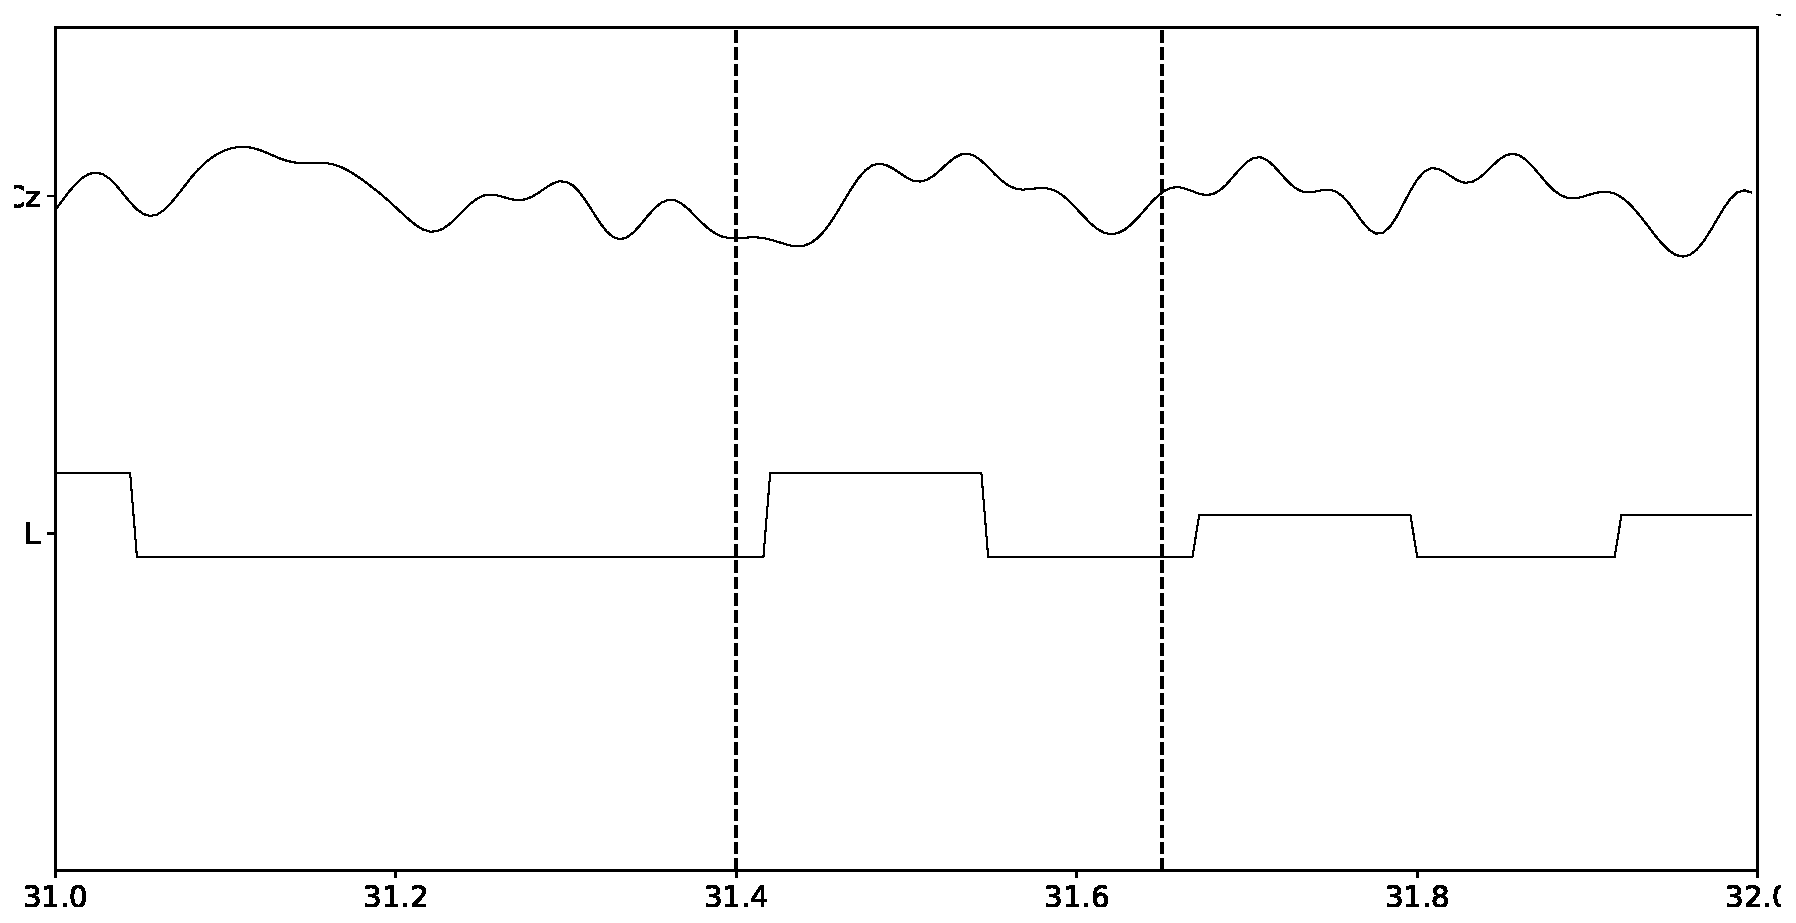
\includegraphics[width=.45\linewidth]{images/nogainzoomhit.eps}}
\subfigure[The same segment with the superimposed template.]{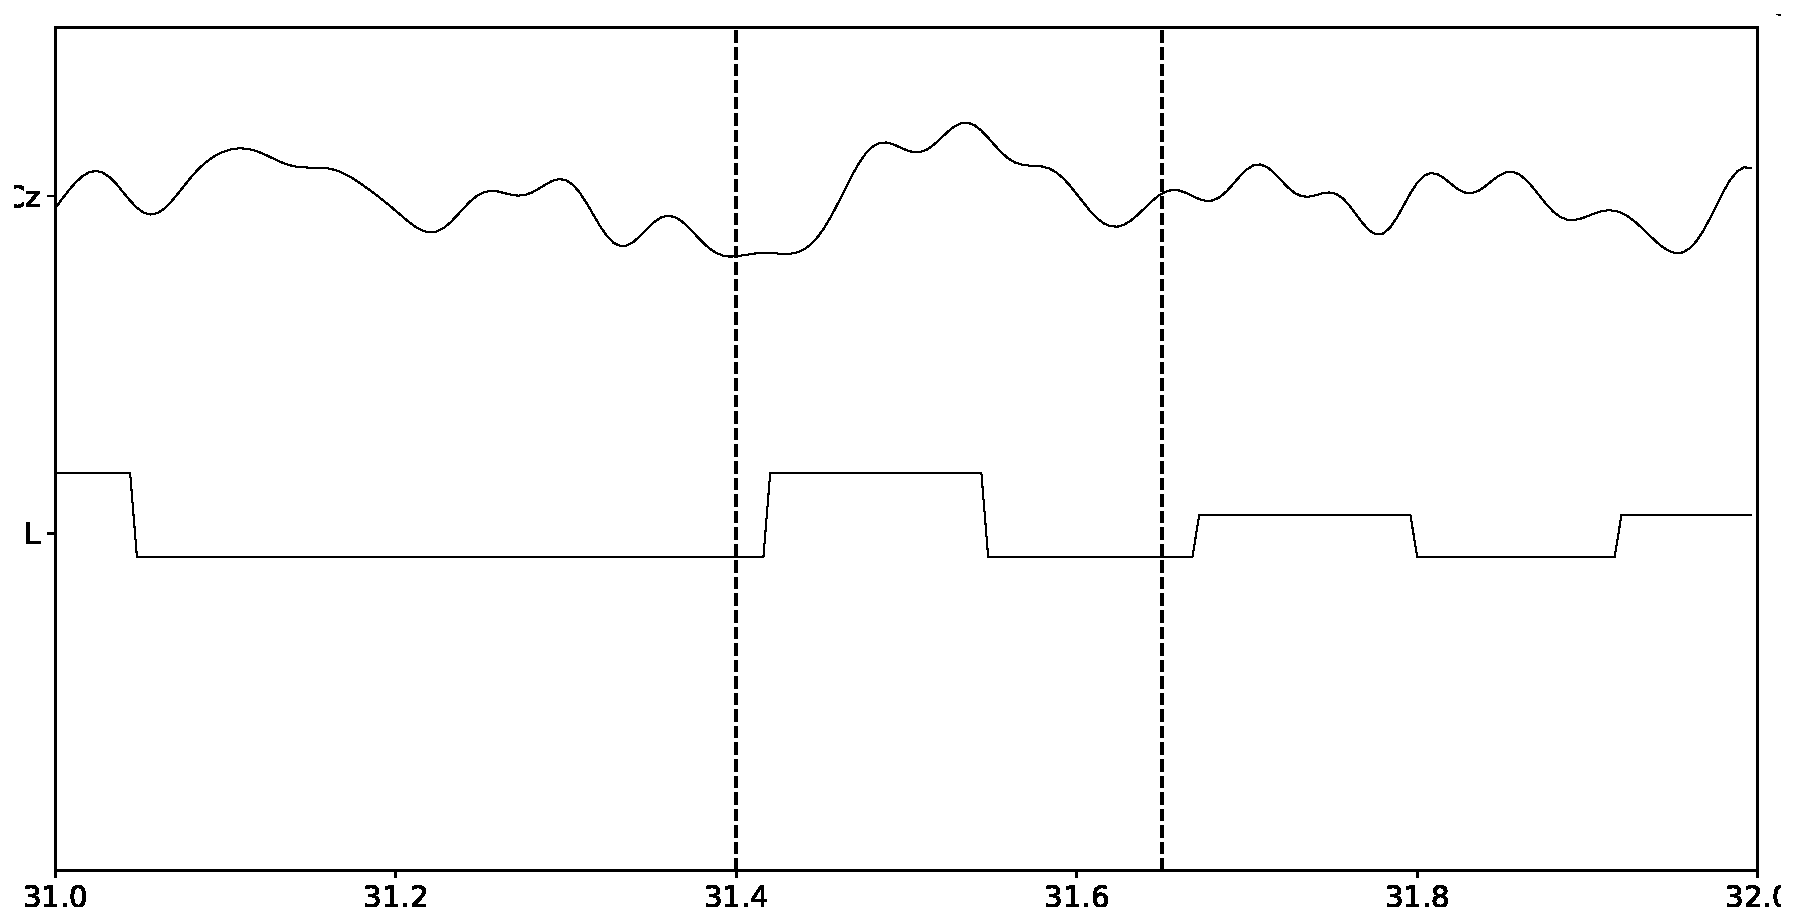
\includegraphics[width=.45\linewidth]{images/singlegainzoomhit.eps}}
\caption{Eight-channel EEG signal without and with the superimposed ERP Template. The channel L, the mark which identifies where to superimpose the P300 ERP, is shown as well as the channel S which identifies the stimulus that was presented. On (c) and (d) the small variation that was introduced by the superimposition of the ERP can be seen enclosed by the vertical bars, where the slope of the bump on subfigure (d) is slightly bigger}
\label{fig:gains}
\end{figure}


%\begin{figure}[H]
%\centering
%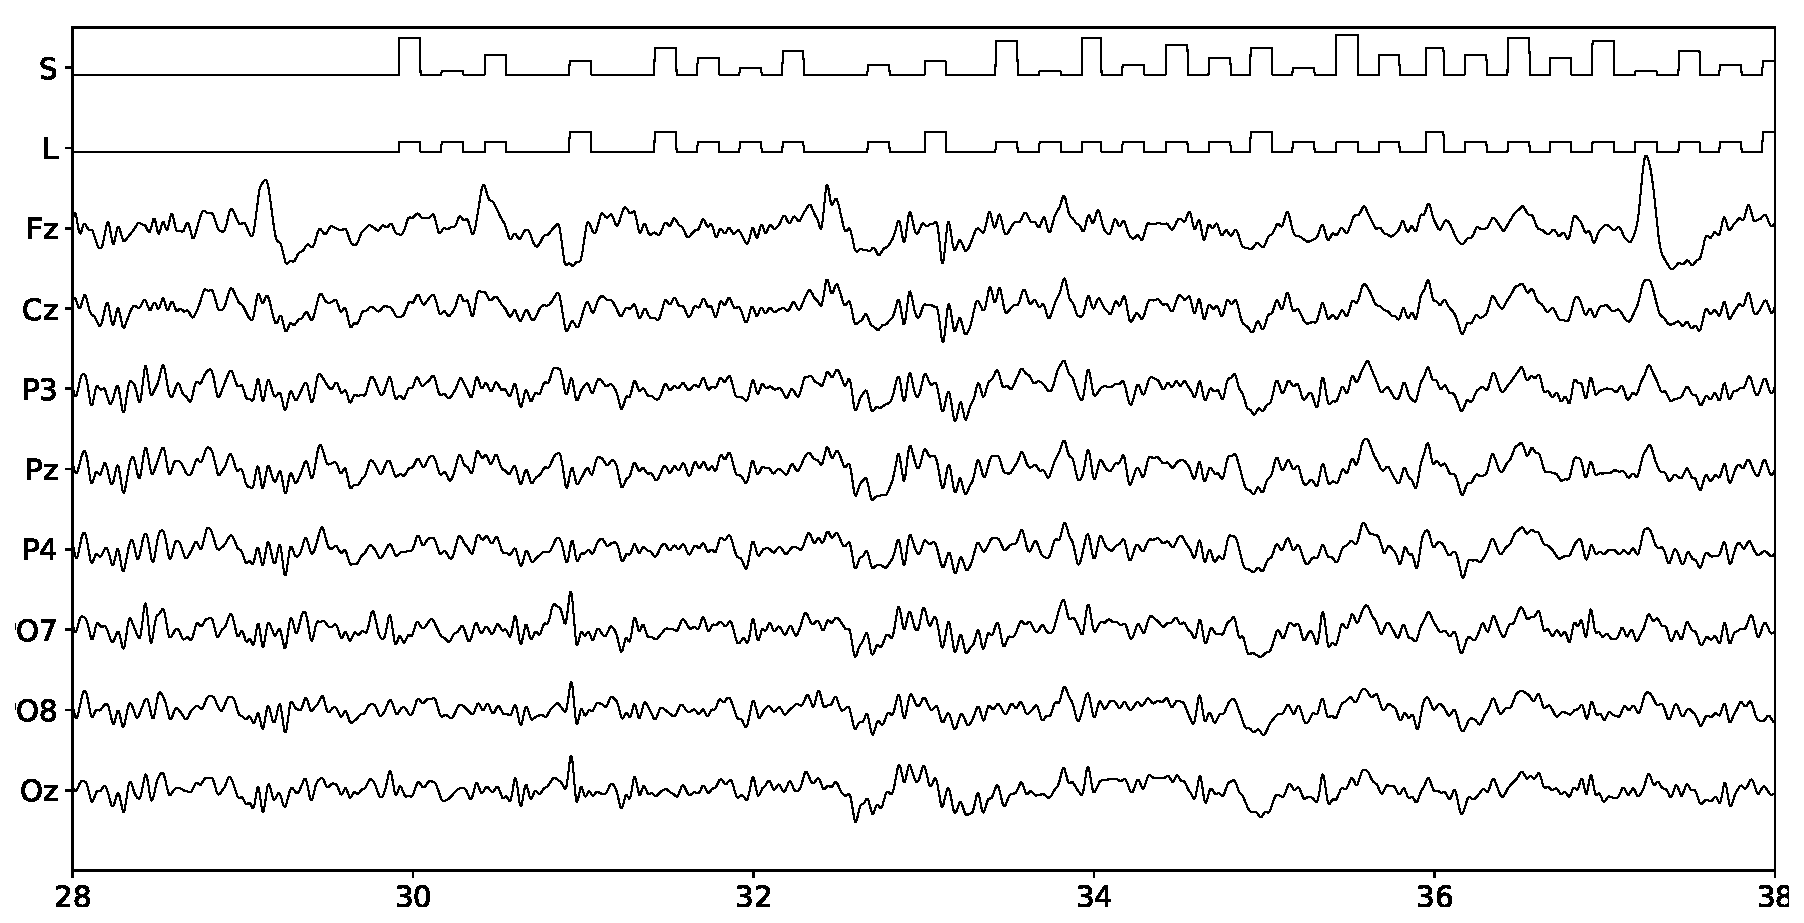
\includegraphics[width=12cm]{images/nogain.eps}
%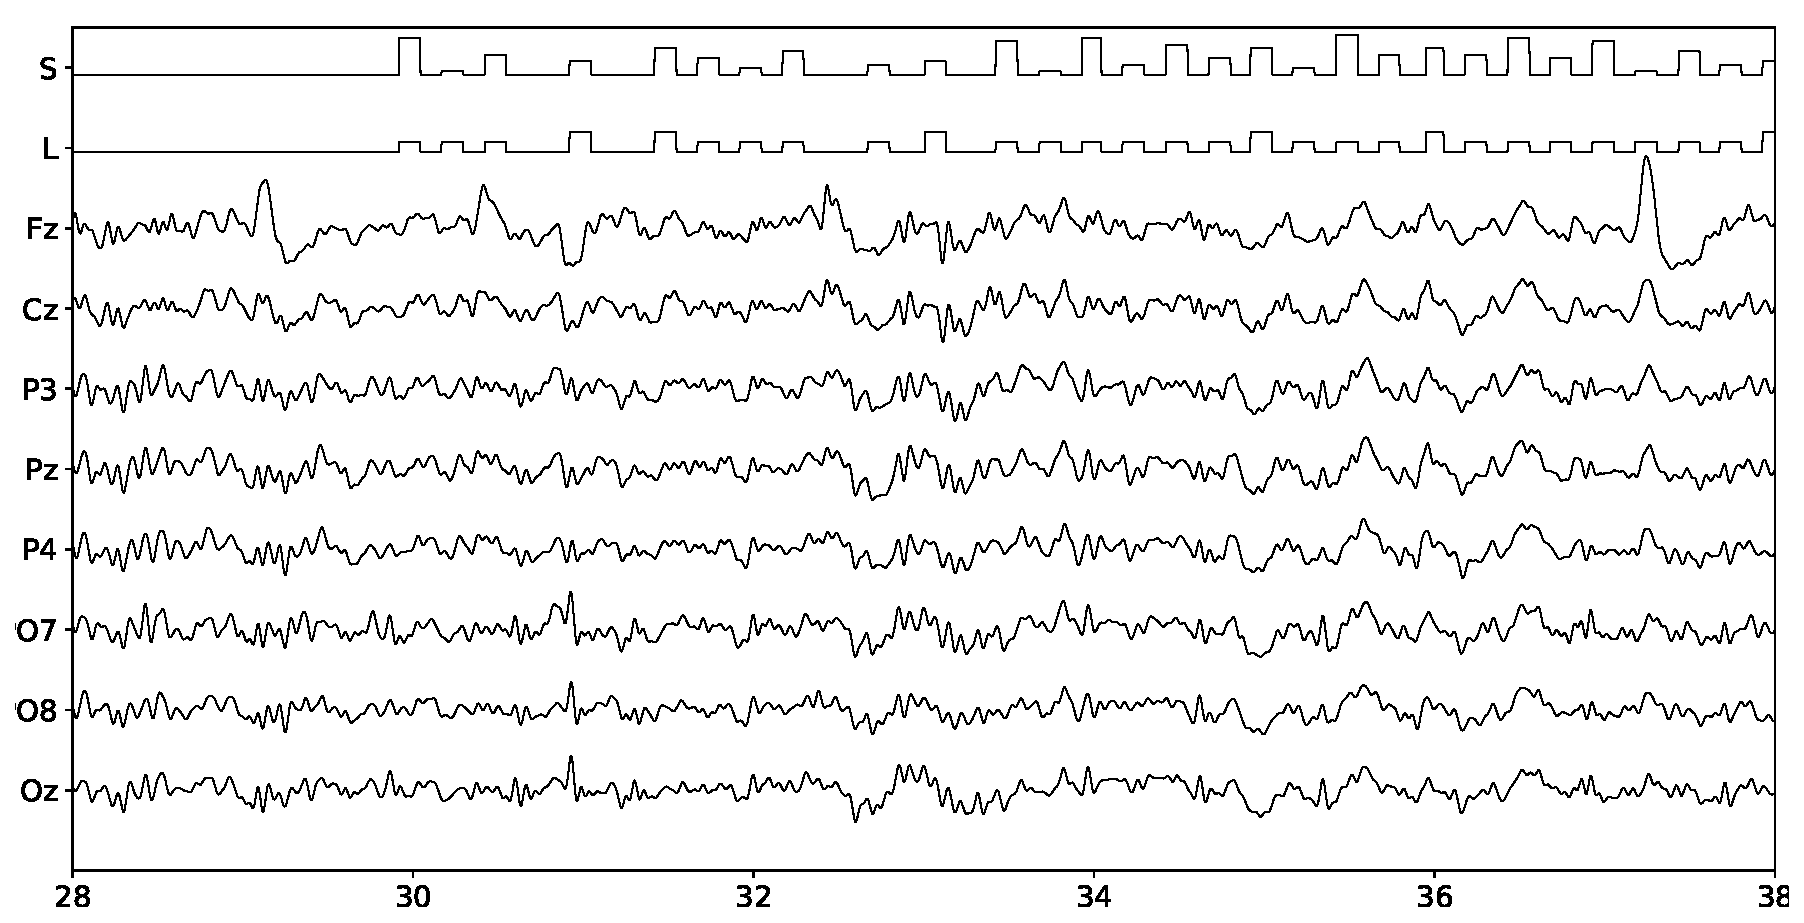
\includegraphics[width=12cm]{images/singlegain.eps}
%\caption{Eight-channel EEG signal superimposed with the ERP Template.  (Left) EEG trace of the original signal. (Right) The same signal segment with the added template.}
%\label{fig:doubleandtriplegain}
%\end{figure}

\begin{figure}[H]
\centering
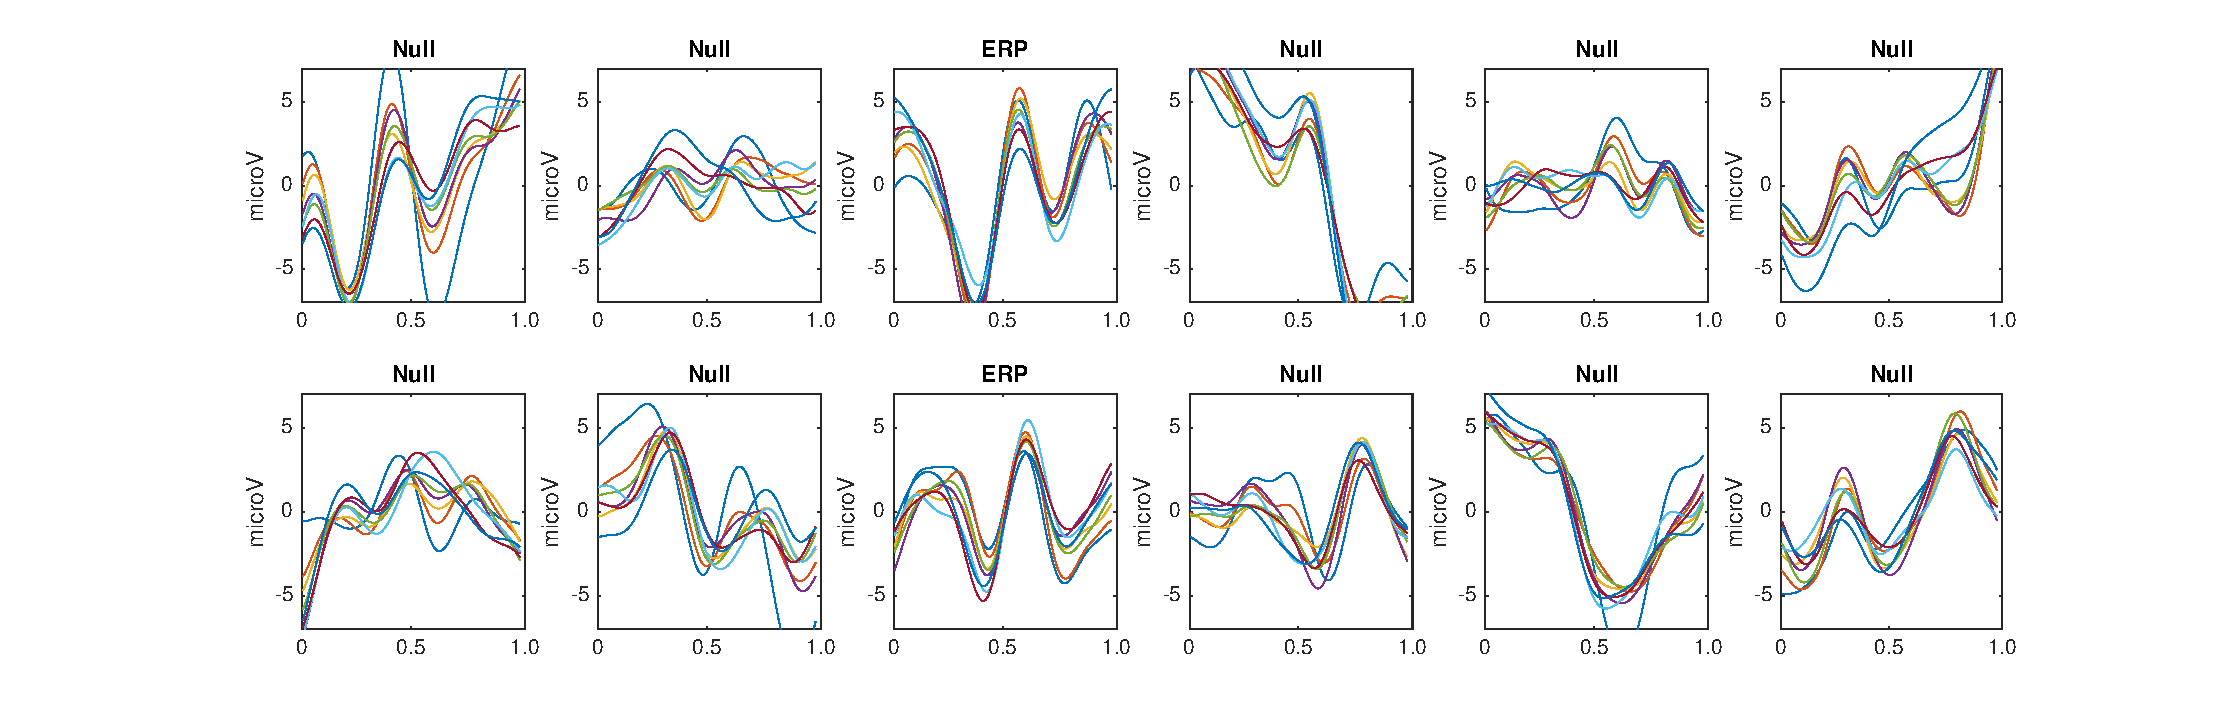
\includegraphics[width=1.0\linewidth]{images/GainCheck.eps}
\caption{Point-to-point averaged signals for the first letter identification trial.  The ERP is superimposed on classes 3 and 9.  Class 3 is obtained while averaging the segments where the row of the speller matrix is intensified whereas class 9 is calculated from the intensification of the corresponding column.}
\label{fig:gaincheck}
\end{figure}

%The averaging procedure aims to extract the superimposed ERP Template and cancel out everything else on each segment.  

\paragraph{Active modality}

The experiment conducted by~\citep{Riccio2013} is replicated on 4 healthy subjects, performing a copy-spelling task with feedback.  In this case, to construct the pseudo-real dataset each template must first be obtained from each subject.  The most prototypical P300 waveform template is selected by visual observation as well.  This template is superimposed to each segment marked as hit on the EEG stream.  The baseline of each segment, on the other hand, is obtained by picking randomly any no hit segment for the same subject.


\subsubsection{Classification} \label{section:classification}

The same classification algorithm based on k-nearest neighbors is used for all the methods~\citep{Boiman2008}.   The experimental protocol used to generated the pseudo-real dataset used in the experiments 1 to 3 is composed of $35$ trials to spell $7$ words of $5$ letters each.  Each trial is composed of $10$ intensification sequences of the $6$ columns and $6$ rows of the Speller Matrix.  Fifteen trials are used to build the dictionary of templates, extracting the averaged EEG segments for the row and column that already contain the P300 ERP, hence shielding $30$ different templates per channel.  Figure~\ref{fig:dictionaryfig} shows the set of templates while using the first $15$ trials of the dataset.

Described algorithms produce a feature $f$ for each EEG segment.  The aim of the classification procedure is to identify for the remaining $20$ trials which of the 6 features $f$ that were obtained for row intensification, labeled by $\{ 1,...,6 \}$, and which of the 6 features for column intensification, named $\{ 7,...,12 \}$ are the ones that elicited the P300 response on the averaged EEG segment. The row number of the matrix can be obtained by doing

\begin{equation}
\hat{row} = \arg \min_{u \in \{1,\dots,6\}} \sum_{i=1}^{k} \left\lVert f_u - q_i \right\rVert ^2
\label{eq:multiclassificationrow}
\end{equation}

\noindent with $q_i$ being the set of k-nearest neighbors of the feature $f_u$ with $u$ varying from $1$ to $6$.  The parameter $k$ represents the number of neighbors chosen from the dictionary of templates.  The column can be obtained in the same way,

\begin{equation}
\hat{col} = \arg \min_{u \in \{7,\dots,12\}} \sum_{i=1}^{k} \left\lVert f_u - q_i \right\rVert ^2.
\label{eq:multiclassificationcol}
\end{equation}

Thus, the letter identification performance can be obtained by measuring the accuracy channel-by-channel at identifying the correct letter on the matrix, coordinated by $ \hat{row} $ and $ \hat{col} $.

%\subsubsection{Parameters}

%The parameters for each method were derived from bibliography were they are introduced 


%Each method has its own set of parameters. To define them an optimization problem was defined and the set of values for each method that achieve the maximum performance value for 

\begin{figure}[H]
\centering
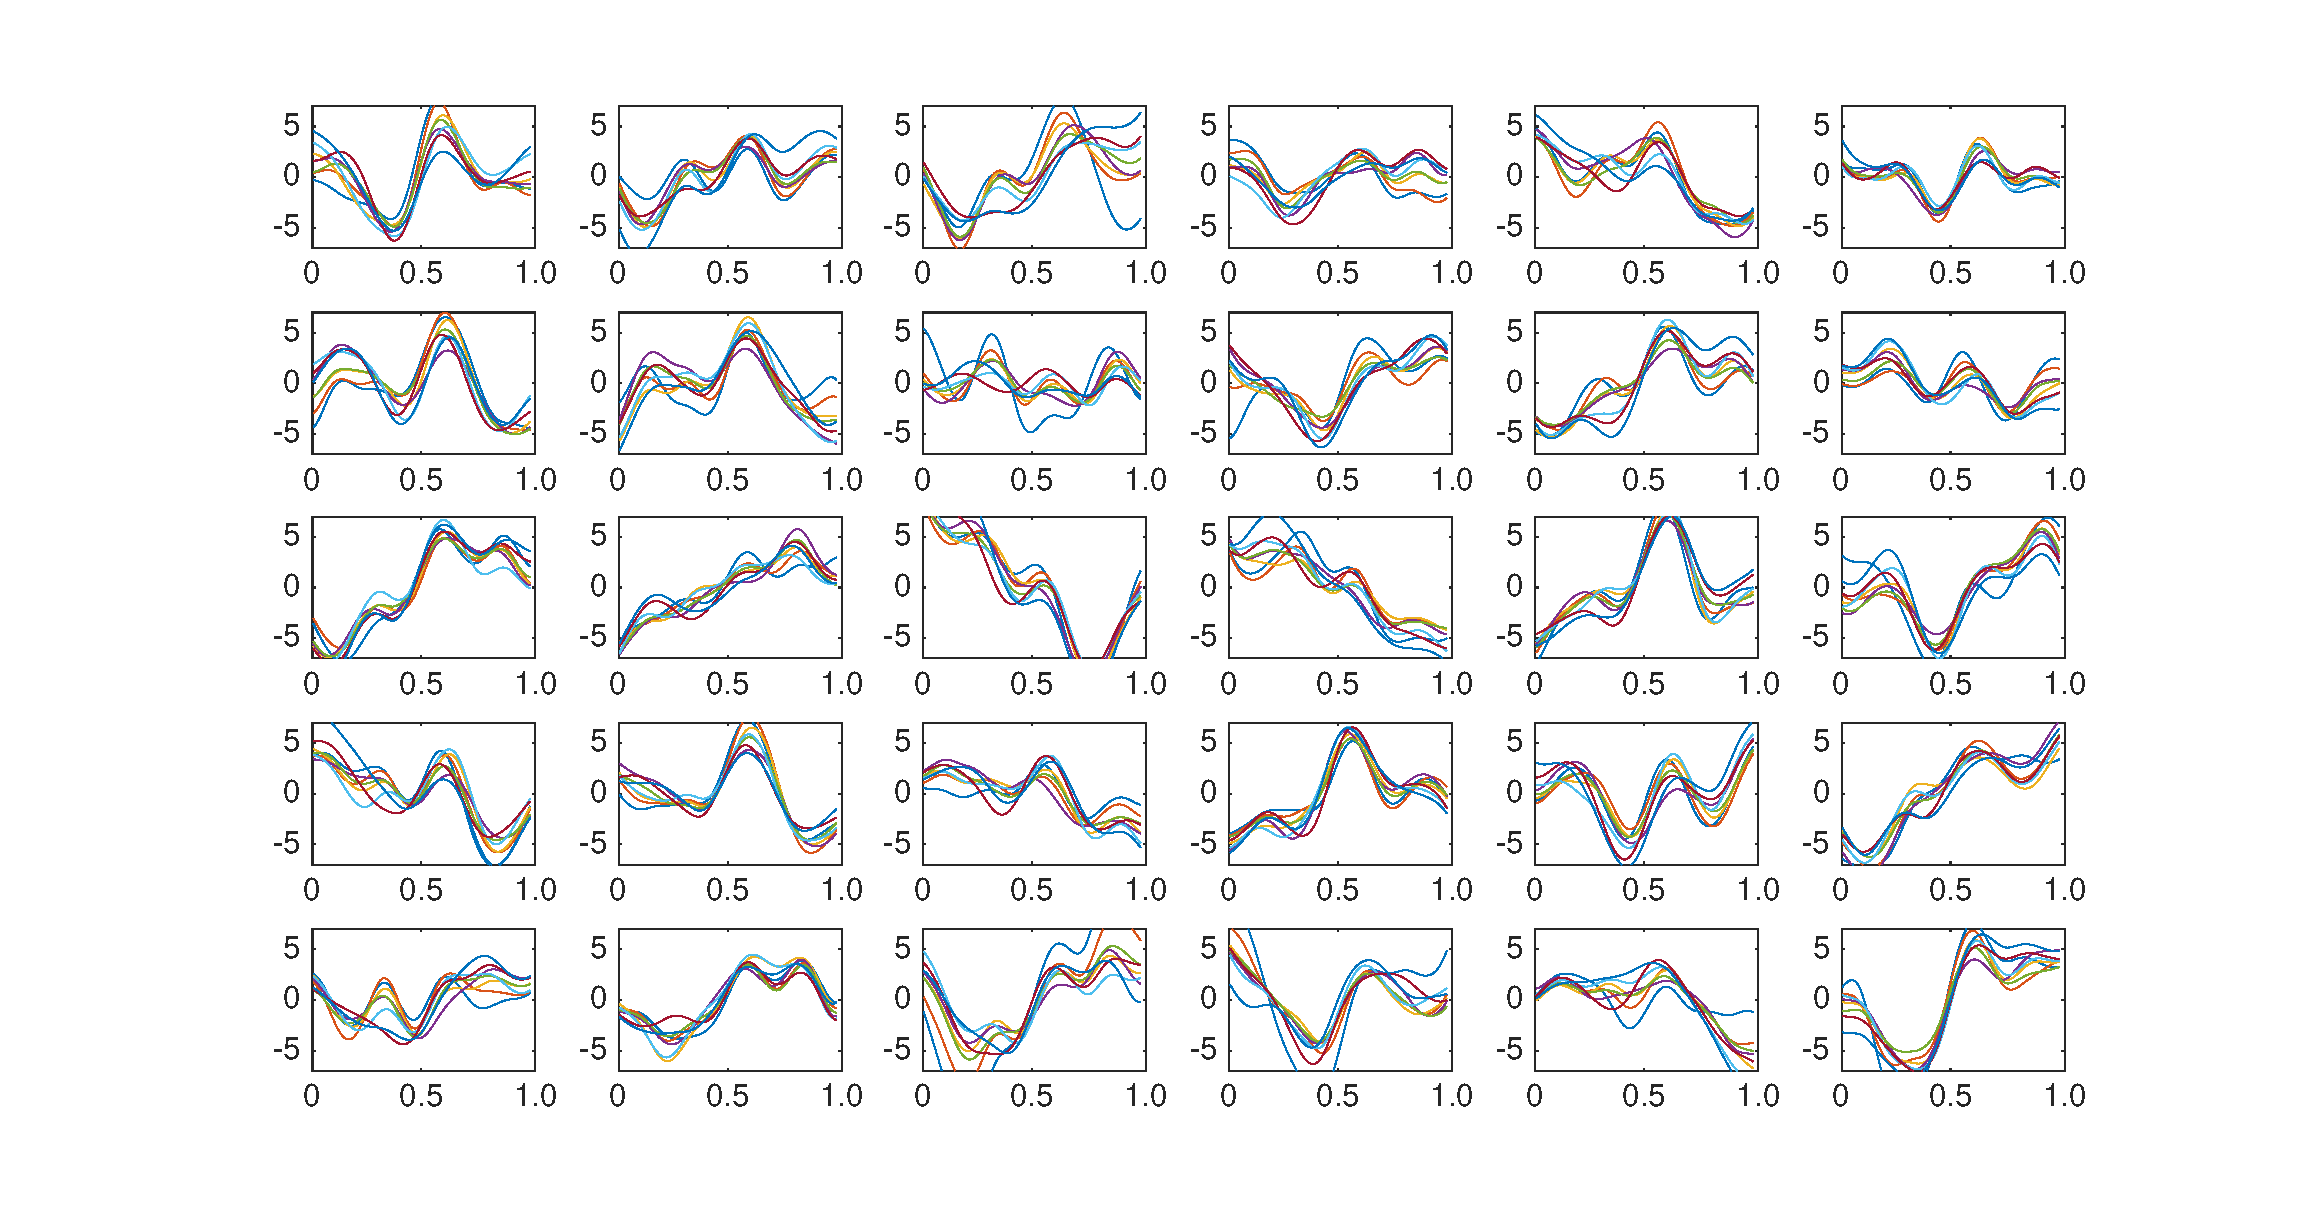
\includegraphics[width=15cm]{images/dictionary.eps}
\caption{Coherently averaged signals containing the superimposed ERP.  Each one is extracted from the 15 first trials (2 signals from each trial, one belonging to the column flashing and the other to row flashing).  These are the templates used to build a dictionary per channel and that are used by the classification algorithm described in \ref{section:classification}.}
\label{fig:dictionaryfig}
\end{figure}


%%%%%%%%%%%%%%%%%%%%%%%%%%%%%%%%%%%%%%%%%%
\section{Results}
\label{section:results}

Results are shown in Table \ref{tab:results} and in Figure \ref{fig:performancetest},\ref{fig:performancetestlatency} and \ref{fig:performancetestamplitude}.  Table \ref{tab:results} shows the  performance while identifying each letter of the standard P300 Speller Matrix, and the channel where the best performance is attained.   Figure \ref{fig:performancetest} shows the performance curves for six algorithms.  Each one represents the percentage of letters that is actually predicted by the algorithms using a cross-validation procedure.  As previously described the data is continuously divided in two sets, where the first 15 letters are used to derive the dictionary of templates while the remaining 20 letters are used to measure the letter identification performance. This is repeated one hundred times, and performances averaged.   

%\begin{table}[H]
%\caption{Speller classification performance obtained for all the waveform-based algorithms: MP Matching Pursuit, SIFT Scale Invariant Feature Transform, PE Permutation Entropy and SHCC Slope Horizontal Code Chain. Additionally, the control algorithm SVM Support Vector Machines is included for comparison.  All the methods process the signal on a channel-by-channel basis, hence the best performing channel is also shown. In this case with absence of null-signals, it can be interpreted as the channel that adds less noise to the ERP template.  All the methods used $10$ intensification sequences to coherently average the trials to obtain the averaged signal. }
%\centering
%%% \tablesize{} %% You can specify the fontsize here, e.g.  \tablesize{\footnotesize}. If commented out \small will be used.
%\begin{tabular}{c|cccc|cccc|cccc|cccc|cccc|cccc|cccc|cccc}
%\toprule
%\textbf{Method}	& \multicolumn{4}{c}{Subject 1} & \multicolumn{4}{c}{Subject 2} & \multicolumn{4}{c}{Subject 3} & \multicolumn{4}{c}{Subject 4} & \multicolumn{4}{c}{Subject 5} & \multicolumn{4}{c}{Subject 6} & \multicolumn{4}{c}{Subject 7} & \multicolumn{4}{c}{Subject 8} \\
%%\cline{3-5} \\
% 	&  \textbf{Channel} & \textbf{Experiment 1} & \textbf{Experiment 2}	& \textbf{Experiment 3}  &  \textbf{Channel} & \textbf{Experiment 1} & \textbf{Experiment 2}	& \textbf{Experiment 3}  &  \textbf{Channel} & \textbf{Experiment 1} & \textbf{Experiment 2}	& \textbf{Experiment 3}  &  \textbf{Channel} & \textbf{Experiment 1} & \textbf{Experiment 2}	& \textbf{Experiment 3}  &  \textbf{Channel} & \textbf{Experiment 1} & \textbf{Experiment 2}	& \textbf{Experiment 3}  &  \textbf{Channel} & \textbf{Experiment 1} & \textbf{Experiment 2}	& \textbf{Experiment 3}  &  \textbf{Channel} & \textbf{Experiment 1} & \textbf{Experiment 2}	& \textbf{Experiment 3}  &  \textbf{Channel} & \textbf{Experiment 1} & \textbf{Experiment 2}	& \textbf{Experiment 3}\\
%\midrule
%MP 1 & PO8  & $67\%$ & $15\%$ & $50\%$  & PO8  & $67\%$ & $15\%$ & $50\%$ & PO8  & $67\%$ & $15\%$ & $50\%$ & PO8  & $67\%$ & $15\%$ & $50\%$ & PO8  & $67\%$ & $15\%$ & $50\%$ & PO8  & $67\%$ & $15\%$ & $50\%$ & PO8  & $67\%$ & $15\%$ & $50\%$ & PO8  & $67\%$ & $15\%$ & $50\%$   \\
%MP 2 & PO7 & $24\%$ & $6\%$ & $10\%$  & PO8  & $67\%$ & $15\%$ & $50\%$ & PO8  & $67\%$ & $15\%$ & $50\%$ & PO8  & $67\%$ & $15\%$ & $50\%$ & PO8  & $67\%$ & $15\%$ & $50\%$ & PO8  & $67\%$ & $15\%$ & $50\%$ & PO8  & $67\%$ & $15\%$ & $50\%$ & PO8  & $67\%$ & $15\%$ & $50\%$ \\
%SIFT  & PO8 & $91\%$ & $18\%$ & $66\%$ & PO8  & $67\%$ & $15\%$ & $50\%$ & PO8  & $67\%$ & $15\%$ & $50\%$ & PO8  & $67\%$ & $15\%$ & $50\%$ & PO8  & $67\%$ & $15\%$ & $50\%$ & PO8  & $67\%$ & $15\%$ & $50\%$ & PO8  & $67\%$ & $15\%$ & $50\%$ & PO8  & $67\%$ & $15\%$ & $50\%$ \\
%PE     & Cz & $61\%$ & $9\%$ & $32\%$ & PO8  & $67\%$ & $15\%$ & $50\%$ & PO8  & $67\%$ & $15\%$ & $50\%$ & PO8  & $67\%$ & $15\%$ & $50\%$ & PO8  & $67\%$ & $15\%$ & $50\%$ & PO8  & $67\%$ & $15\%$ & $50\%$ & PO8  & $67\%$ & $15\%$ & $50\%$ & PO8  & $67\%$ & $15\%$ & $50\%$ \\
%SHCC & P4 & $98\%$ & $31\%$ & $80\%$ & PO8  & $67\%$ & $15\%$ & $50\%$ & PO8  & $67\%$ & $15\%$ & $50\%$ & PO8  & $67\%$ & $15\%$ & $50\%$ & PO8  & $67\%$ & $15\%$ & $50\%$ & PO8  & $67\%$ & $15\%$ & $50\%$ & PO8  & $67\%$ & $15\%$ & $50\%$ & PO8  & $67\%$ & $15\%$ & $50\%$ \\
%SVM     & PO8  & $78\%$ & $7\%$ & $53\%$ & PO8  & $67\%$ & $15\%$ & $50\%$ & PO8  & $67\%$ & $15\%$ & $50\%$ & PO8  & $67\%$ & $15\%$ & $50\%$ & PO8  & $67\%$ & $15\%$ & $50\%$ & PO8  & $67\%$ & $15\%$ & $50\%$ & PO8  & $67\%$ & $15\%$ & $50\%$ & PO8  & $67\%$ & $15\%$ & $50\%$ \\
%\bottomrule
%\end{tabular}
%\label{tab:results}
%\end{table}


Figure \ref{fig:performancetestlatency} shows the same results for the Experiment 2, where a noisy latency lag was included.   Finally, Figure \ref{fig:performancetestamplitude} represents the performance values obtained for the Experiment 3, when the amplitude of the P3b component of the template is randomly attenuated.  

\begin{figure}[H]
\centering
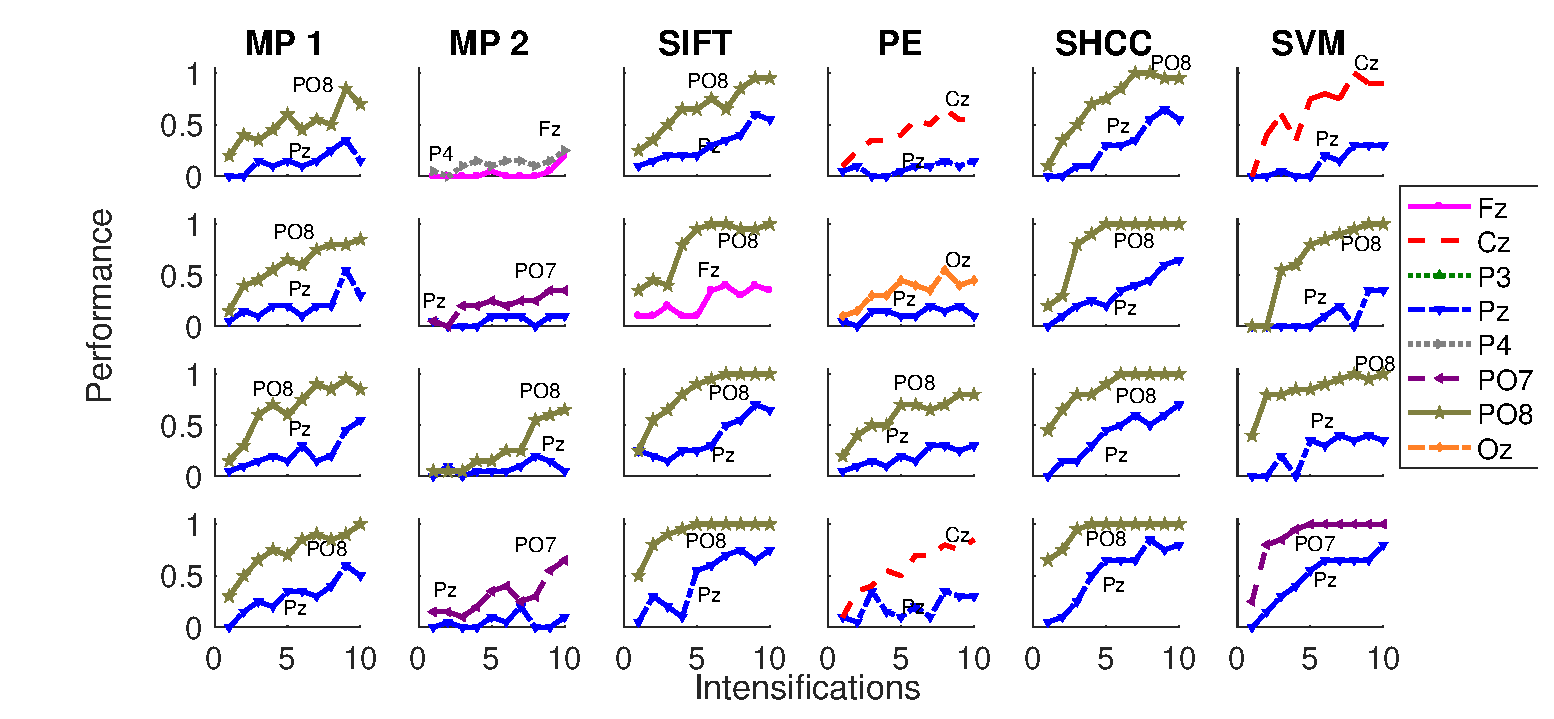
\includegraphics[width=7.5cm]{images/1-1.eps}
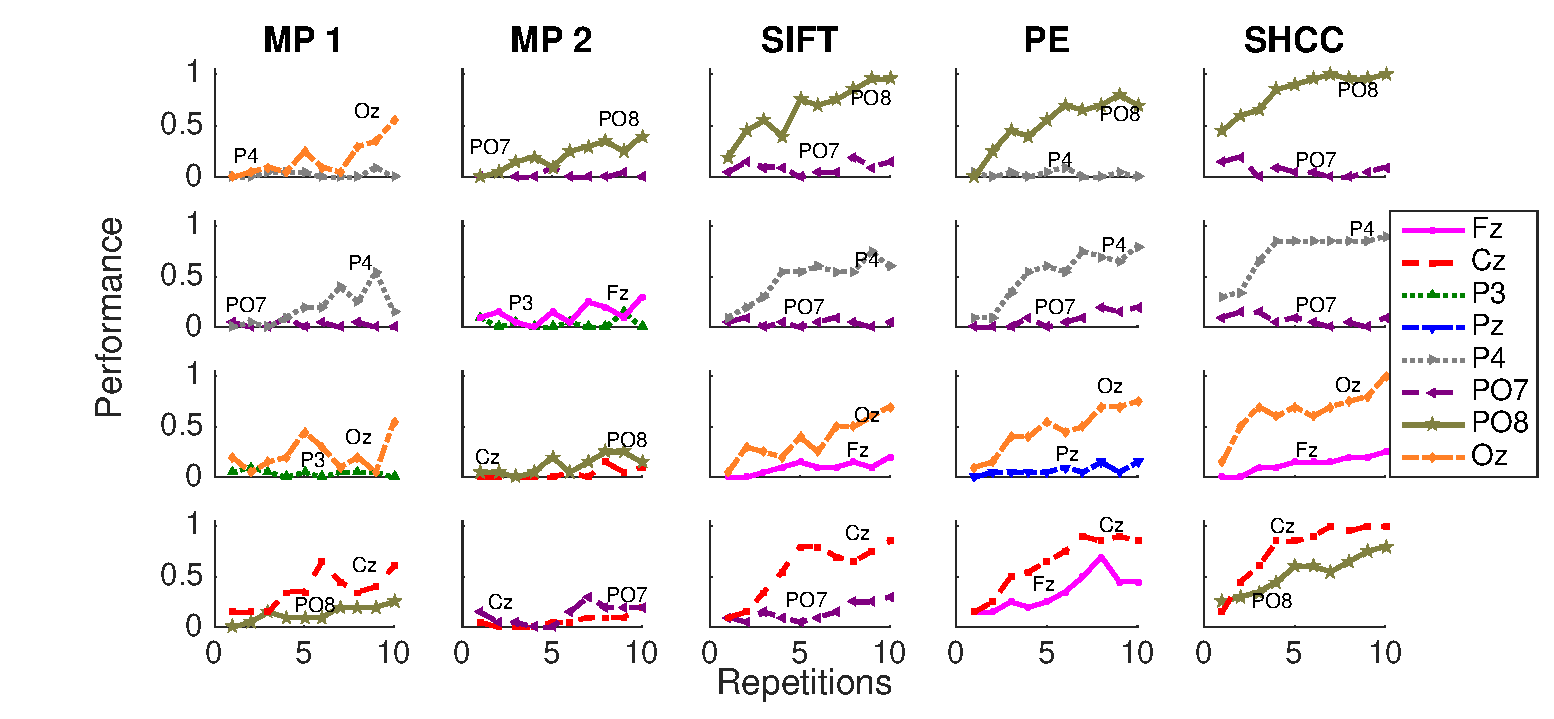
\includegraphics[width=7.5cm]{images/2-1.eps}
\caption{Speller performance obtained for each method for the Experiment 1.  Y-axis shows performance accuracy while X-axis shows the number of intensification sequences used to calculate the point-to-point signal average.}
\label{fig:performancetest}
\end{figure}


\begin{figure}[H]
\centering
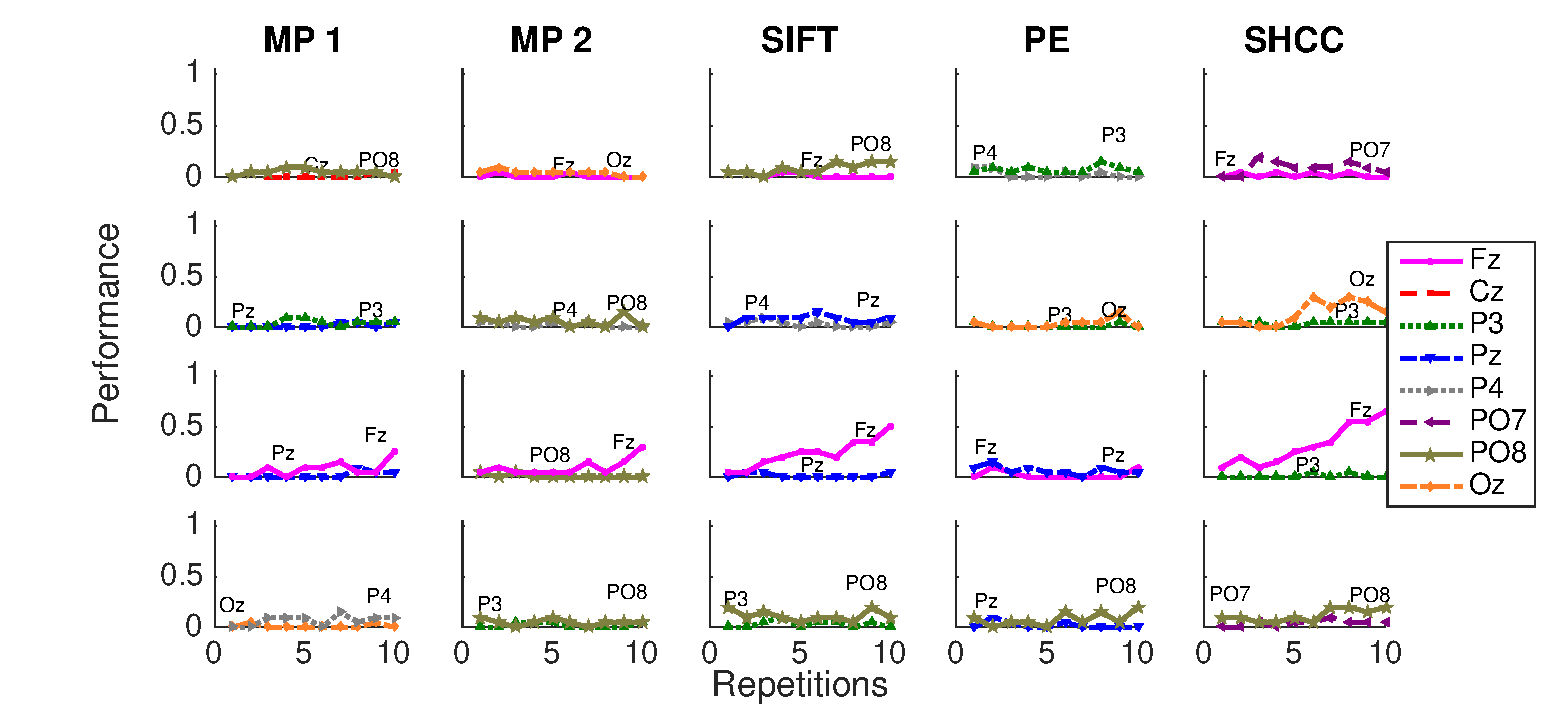
\includegraphics[width=7.5cm]{images/1-2.eps}
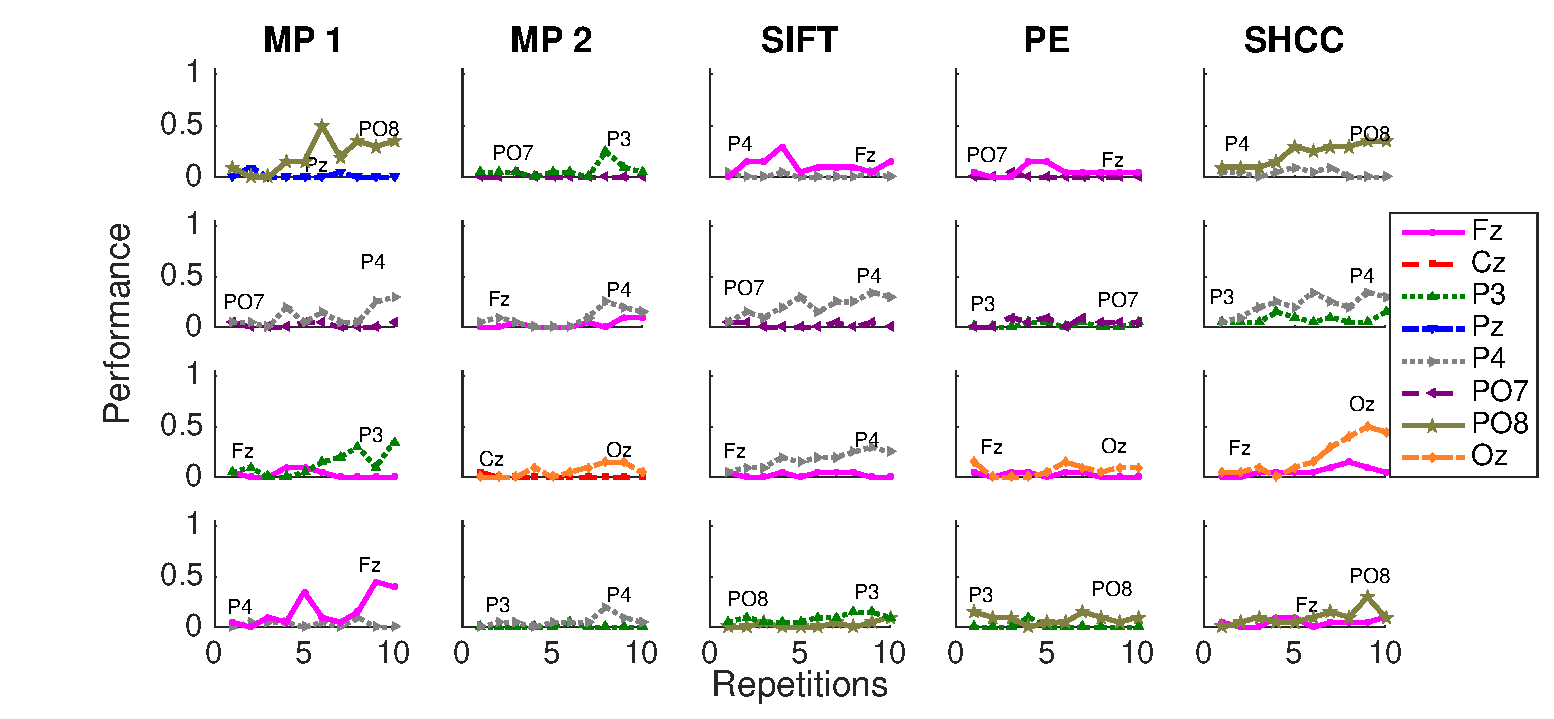
\includegraphics[width=7.5cm]{images/2-2.eps}
\caption{Speller performance obtained for each method while latencies are artificially added to each single-intensification segment corresponding to the Experiment 2.  The achieved performance is significantly reduced for all methods. Y-axis shows letter identification performance while X-axis shows the number of intensification sequences used to calculate the ensemble average.}
\label{fig:performancetestlatency}
\end{figure}


\begin{figure}[H]
\centering
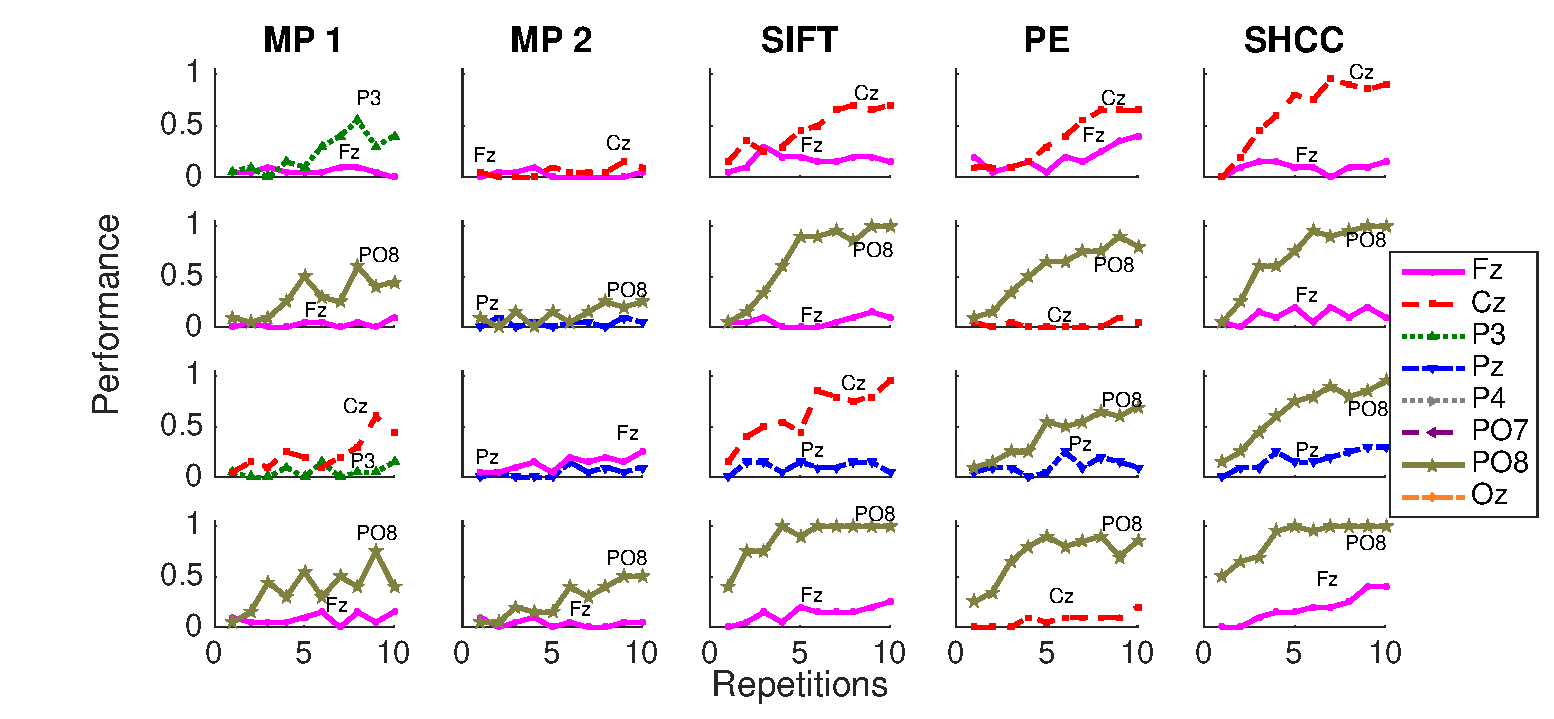
\includegraphics[width=7.5cm]{images/1-3.eps}
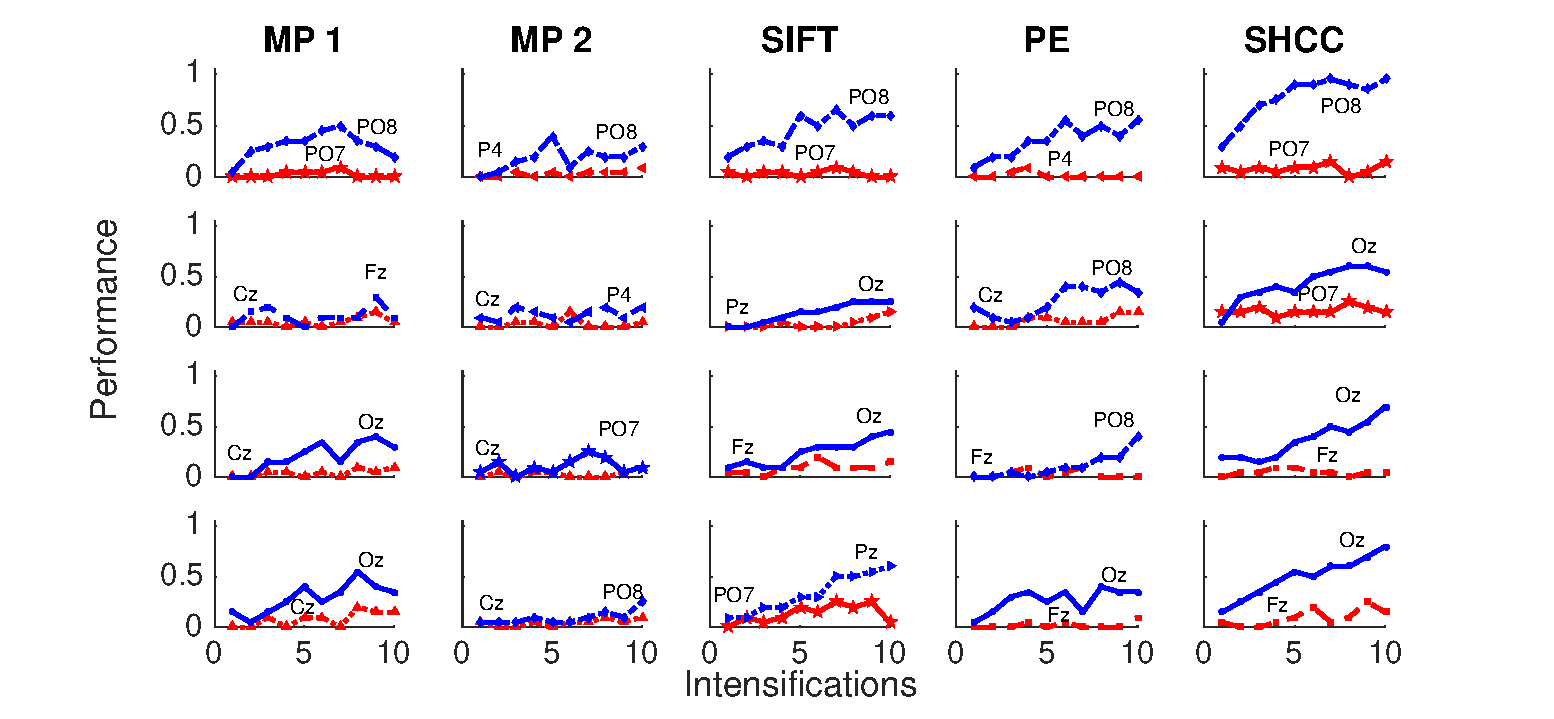
\includegraphics[width=7.5cm]{images/2-3.eps}
\caption{Speller performance obtained for the Experiment 3 while the amplitudes of the P3b component of the superimposed ERP is randomly reduced. Y-axis shows performance accuracy while X-axis shows the number of intensification sequences.}
\label{fig:performancetestamplitude}
\end{figure}

Furthermore, results obtained for the dataset BCI Competition 2003 IIb are shown in Figures \ref{fig:performancebcicompetition} and in Table~\ref{tab:bcicompetitionresults}.  For this experiment the number of available intensification sequences is 15.

\begin{figure}[H]
\centering
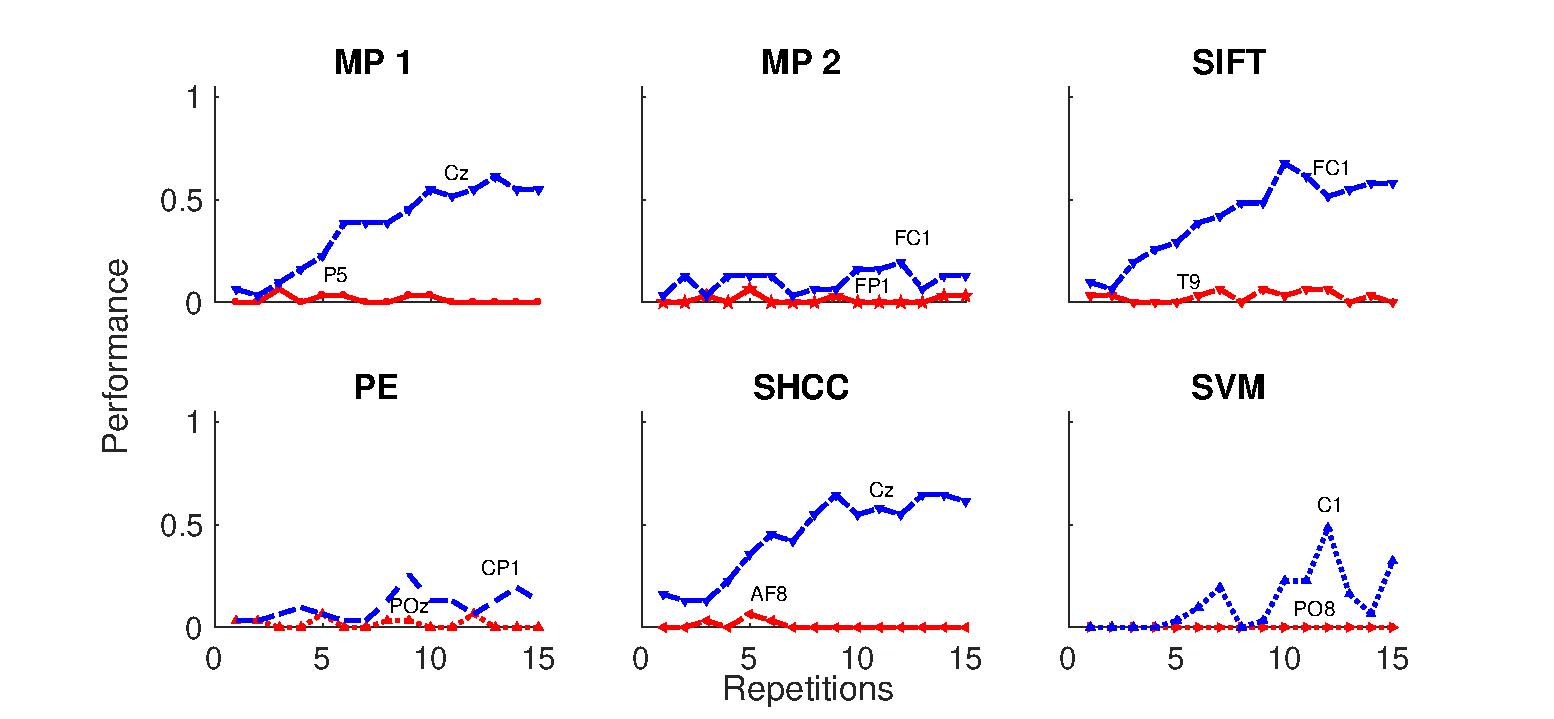
\includegraphics[width=15cm]{images/PerformanceBCICompetition.eps}
\caption{Speller performance obtained for the Dataset IIb of the BCI Competition II (2003) for each one of the algorithms.  An offline BCI Simulation is performed using the first $42$ trials as training and the remaining $31$ as testing.  The horizontal axis show the number of intensification sequences, from $0$ to $15$ for this dataset, while the vertical axis show the performance rate.}
\label{fig:performancebcicompetition}
\end{figure}


\begin{table}[H]
\caption{Speller classification performance obtained for the dataset IIb of the BCI Competition II (2003) for each one of the algorithms using $15$ repetitions of intensification sequences. The first $42$ trials are used for training to build the template dictionary and the remaining $31$ for testing. The channel where the best performance is attained, is also shown. }
\centering
%% \tablesize{} %% You can specify the fontsize here, e.g.  \tablesize{\footnotesize}. If commented out \small will be used.
\begin{tabular}{ccc}
\toprule
\textbf{Method}	& \textbf{Channel} &  \textbf{Performance} \\
\midrule
MP 1 & FC2  & $50\%$ \\
MP 2 & CPz & $22\%$ \\
SIFT  & Cz & $67\%$ \\
PE     & PO8 & $22\%$ \\
SHCC & Cz & $61\%$ \\
SVM     & C1  & $32\%$ \\
\bottomrule
\end{tabular}
\label{tab:bcicompetitionresults}
\end{table}


%%%%%%%%%%%%%%%%%%%%%%%%%%%%%%%%%%%%%%%%%%
\section{Discussion}
\label{section:discussion}

A significant reduction of performance was found when latency noise is added (Experiment 1 vs 2, Wilcoxon rank sum test, one tail, with $p=0.0022$).  The latency noise reduces the information contained in the averaged signal, mainly due to the invalidation of the SNR enhancement performed by the signal averaging procedure.  This reduction alters the obtained shape of the waveform of the ERP and impacts on the performances regardless of the method. On the other hand, all the algorithms show some resistance to noise in peak amplitudes of the main component. This is shown by the similarities of obtained results between the Experiment 1 and 3 (Wilcoxon rank sum test, two tails, not rejected with $p=0.1797$).

\begin{table}[H]
\caption{Statistical Analysis Tests }
\centering
%% \tablesize{} %% You can specify the fontsize here, e.g.  \tablesize{\footnotesize}. If commented out \small will be used.
\begin{tabular}{ccc}
\toprule
\textbf{Comparison}	& \textbf{Statistical Method} &   \textbf{p-value} \\
\midrule
Experiment 1 vs. 2 & Wilcoxon rank sum test, one tail  & $0.0022$ \\
Experiment 1 vs. 3 & Wilcoxon rank sum test, two tails not rejected & $0.1797$ \\
\bottomrule
\end{tabular}
\label{tab:statisticalanalysis1}
\end{table}


\begin{table}[H]
\caption{Statistical Analysis Tests  - Multiple comparisons}
\centering
%% \tablesize{} %% You can specify the fontsize here, e.g.  \tablesize{\footnotesize}. If commented out \small will be used.
\begin{tabular}{ccc}
\toprule
\textbf{Comparison}	& \textbf{Statistical Method} &   \textbf{p-value} \\
\midrule
SHCC & MP-1, MP-2  & $0.05$ \\
SIFT   & MP-2, PE       & $0.1797$ \\
SVM   & MP-2             & $0.1797$ \\
\bottomrule
\end{tabular}
\label{tab:statisticalanalysis2}
\end{table}

A two-way balanced Quade test was performed to evaluate the performance's differences for the three experiments and for the six methods.  Difference among the method's letter identification rates were found with $p=0.0019$.  The methods \textit{SHCC}, \textit{SIFT}, \textit{MP-1} performed much better than the other algorithms, including \textit{SVM}.  By making multiple comparisons at a level  $0.05$, significant differences are found between \textit{SHCC} vs MP-1,MP-2, PE and SVM, between \textit{SIFT} vs. MP-2 and PE, and between \textit{SVM} and MP-2.

Additionally, using a straightforward dictionary of templates for \textit{MP-1} proved more beneficial in terms of performance than the approach of using a Hilbert base of Wavelets atoms on \textit{MP-2} (significant differences between MP-1 vs MP-2).  Either applying latency noise or amplitude noise, the method based on the signal's templates instead of using their coefficients achieve much better character identification rates.  

Regarding results produced for the public and real dataset IIb of P300 ERP from the Berlin BCI Competition II (2003), the obtained character identification rate is above theoretical chance level, and for some algorithms close to the usable threshold of $70\%$~\citep{Kathner2017}.  When the character identification rate reaches this level of performance, the usage of word predicting algorithms allows to implement practical speller applications.  Results for this competition have shown perfect classification with tailored algorithm.  This level is also similar to the performance obtained for the Experiment 3, which represents coincidentally the more realistic scenario for the pseudo-real dataset.  It is important to remark that the algorithms presented here analyze the waveform structure of a single-channel signal~\citep{Rakotomamonjy2008,Gribonval2008}.  

%%%%%%%%%%%%%%%%%%%%%%%%%%%%%%%%%%%%%%%%%%
\section{Conclusion}
\label{section:conclusion}

The purpose of this work is threefold, (1) raise awareness about the utility of using automatic waveform-based methods to study EEG signals, (2) to provide an overview of the state-of-the-art of those methods, and (3) to compare those methods and verify if it is possible to obtain acceptable classification performances based exclusively on the signal's waveform.

We verified that similar performance results are obtained for the methods \textit{SHCC}, \textit{SIFT} and \textit{MP-1} and that it is possible to obtain discriminating information from the underlying signal based exclusively on an automated method of processing the waveforms.  This brings the possibility to use these techniques to implement intelligible automatic detection procedures due to the fact that they are based on metrics which can be visually verified.  

Further work should be conducted in terms of a multichannel meaningful extension of these waveform-based methods~\citep{Gribonval2008}. Moreover, the possibilities of finding overcomplete dictionaries for matching pursuit sparse representation based on obtained signal templates, could also be considered an area of future improvement.

%How much is it possible to classify and implement a P300 ERP Speller using only the waveform structure of the signal ? Which algorithm perform better at this even when segment latency variations and component amplitudes issues are present ?

One of the main goals of the BCI discipline is to provide assistance to patients and to provide alternative tools to be used in diagnostics and rehabilitation procedure.  This requires a clinical focus which is often neglected in BCI research~\citep{Chavarriaga2017}.  At the same time, BCI reliability is yet an unfulfilled goal in this discipline~\citep{WolpawJonathanR2012}. The convenience of analyzing or including metrics about the shape of the EEG, is that clinical EEG diagnosis may support a vast set of already understood knowledge which is based on identifying EEG patterns by their shape and that can steer towards a more robust implementation of BCI devices.

%The conventional clinical method of observing the waveform is understood to be subjective and laborious because results depend on the technicians' experience and expertise.   At the same time, it is a subjective time-consuming task, with long-learning curves, requires specialized personnel, and it has significant error rates~\citep{Tjepkema-Cloostermans2018}.  These problems has pushed for the adoption of more automated means of decoding the signals~\citep{Thakor2004}.   This trend pointed to the initial development of quantitative EEG, which however didn't replaced clinically the traditional approach which is still widespread: the Gold standard in clinical EEG is still \textit{Eye Ball}~\citep{Wulsin2011,Tjepkema-Cloostermans2018}.  

We believe that the adoption of a \textit{hybrid} methodology which can process the signal automatically, but at the same time, maintains an inherent intelligible property~\citep{j2018challenge} that can be mapped to existing procedures, and above all, can maintain the clinician trust on the system behavior is beneficial to Clinical Practice, Neuroscience and BCI research. 

%These methods have the advantage that they can map a visual component with a clinical meaning to a feature with an objective representation. Compound classifiers or ensemble of features can be explored.  Successful approaches in Computer Vision or Pattern Recognition in other areas use them~\citep{Criminisi2013} with a significant enhancement of the classification performances~\citep{Gu2012}.

% This is an important area for future study.

Another benefit of these methodologies is that they have a potential universal applicability.  As they are only analyzing waveform, they can be explored in other disciplines where the structure or shape of the waveform is of relevance.  Analyzing signals by their waveforms is relative common in chemical analysis~\citep{Skoog2000}, seismic analysis in Geology~\citep{Owens1984}, and quantitative financial analysis.  Electrocardiogram EKG, on the other hand, has been extensively processed and studied analyzing the waveform structure~\citep{Stockman1976}.
%Additionally, the same problem can be found in Intelligent Character Recognition.

%Berger H: tiber das Elektrenkephalogramm des Menschen, Archiv Psychiatr, 87 (1929) pp. 527-570.

%%%%%%%%%%%%%%%%%%%%%%%%%%%%%%%%%%%%%%%%%%
%\subsection{Subsection}
%
%\subsubsection{Subsubsection}
%
%Bulleted lists look like this:
%\begin{itemize}[leftmargin=*,labelsep=4mm]
%\item	First bullet
%\item	Second bullet
%\item	Third bullet
%\end{itemize}
%
%Numbered lists can be added as follows:
%\begin{enumerate}[leftmargin=*,labelsep=3mm]
%\item	First item
%\item	Second item
%\item	Third item
%\end{enumerate}
%
%The text continues here.



%%%%%%%%%%%%%%%%%%%%%%%%%%%%%%%%%%%%%%%%%%
\vspace{6pt} 

%%%%%%%%%%%%%%%%%%%%%%%%%%%%%%%%%%%%%%%%%%
%% optional
%\supplementary{The following are available online at www.mdpi.com/link, Figure S1: title, Table S1: title, Video S1: title.}

%%%%%%%%%%%%%%%%%%%%%%%%%%%%%%%%%%%%%%%%%%
\acknowledgments{This project was supported by the ITBACyT-15 funding program issued by ITBA University. We would like to thank to Dr. Valentina Unakafova for providing the Permutation Entropy algorithm and to Dr. Montserrat-Alvarado González for providing the source code and a detailed description of the SHCC algorithm.}

%We would like to thank to Dr. Jian Zhang for providing details of the MIDS algorithm, to Dr. Valentina Unakafova for providing the Permutation Entropy algorithm 

%%%%%%%%%%%%%%%%%%%%%%%%%%%%%%%%%%%%%%%%%%
\authorcontributions{This projects is part of a the first author's PhD Thesis which is directed by Juan Miguel Santos and codirected by Ana Julia Villar.}

%%%%%%%%%%%%%%%%%%%%%%%%%%%%%%%%%%%%%%%%%%
%\conflictofinterests{The authors declare no conflict of interest.} 

%%%%%%%%%%%%%%%%%%%%%%%%%%%%%%%%%%%%%%%%%%
%% optional
\abbreviations{The following abbreviations are used in this manuscript:\\

\noindent EEG: electroencephalography\\
BCI: Brain Computer Interfaces\\
BMI: Brain Machine Interfaces\\
BNCI: Brain-Neural Computer Interfaces\\
SNR: Signal to Noise Ratio\\
CNS: Central Nervous System\\
DC: Direct Current\\
ERP: Event-Related Potential\\
P300: Positive deflection of an Event-Related Potential which occurs 300 ms after onset of stimulus\\
ITR: Information Transfer Rate\\
BTR: Bit Transfer Rate\\
SIFT: Scale Invariant Feature Transform\\
SHCC: Slope Horizontal Chain Code\\
PE: Permutation Entropy\\
MP: Matching Pursuit\\
ICU: Intensive Care Unit\\
EKG: Electrocardiogram\\
PAA:Period Amplitude Analysis\\
SVM:Support Vector Machine
}

%%%%%%%%%%%%%%%%%%%%%%%%%%%%%%%%%%%%%%%%%%
%% optional
%\appendixtitles{no} %Leave argument "no" if all appendix headings stay EMPTY (then no dot is printed after "Appendix A"). If the appendix sections contain a heading then change the argument to "yes".
%\appendixsections{multiple} %Leave argument "multiple" if there are multiple sections. Then a counter is printed ("Appendix A?). If there is only one appendix section then change the argument to ?one? and no counter is printed (?Appendix?).
%\appendix
%\section{}
%The appendix is an optional section that can contain details and data supplemental to the main text. For example, explanations of experimental details that would disrupt the flow of the main text, but nonetheless remain crucial to understanding and reproducing the research shown; figures of replicates for experiments of which representative data is shown in the main text can be added here if brief, or as Supplementary data. Mathemtaical proofs of results not central to the paper can be added as an appendix.
%
%\section{}
%All appendix sections must be cited in the main text. In the appendixes, Figures, Tables, etc. should be labeled starting with `A', e.g., Figure A1, Figure A2, etc. 

%%%%%%%%%%%%%%%%%%%%%%%%%%%%%%%%%%%%%%%%%%
% Citations and References in Supplementary files are permitted provided that they also appear in the reference list here. 
\bibliographystyle{mdpi}

%=====================================
% References, variant A: internal bibliography
%=====================================
%\renewcommand\bibname{References}
%\begin{thebibliography}{999}
% Reference 1
%\bibitem{ref-journal}
%Lastname, F.; Author, T. The title of the cited article. {\em Journal Abbreviation} {\bf 2008}, {\em 10}, 142-149.
% Reference 2
%\bibitem{ref-book}
%Lastname, F.F.; Author, T. The title of the cited contribution. In {\em The Book Title}; Editor, F., Meditor, A., Eds.; Publishing House: City, Country, 2007; pp. 32-58.
%\end{thebibliography}

%=====================================
% References, variant B: external bibliography
%=====================================
\bibliography{brainscience}

%%%%%%%%%%%%%%%%%%%%%%%%%%%%%%%%%%%%%%%%%%
%% optional
%\sampleavailability{Samples of the compounds ...... are available from the authors.}

%%%%%%%%%%%%%%%%%%%%%%%%%%%%%%%%%%%%%%%%%%
\end{document}